%%%%%%%%%%%%%%%%%%%%%%%%
\chapter{Revisão Sistemática da Literatura}\label{trabRelac}
%%%%%%%%%%%%%%%%%%%%%%%%

Diante dos desafios impostos pela alta dimensionalidade em classificadores associativos, especialmente relacionados à explosão combinatória do número de \textit{itemsets} candidatos e de regras geradas, torna-se fundamental investigar estratégias que possam mitigar tais limitações. Nesse contexto, a seleção de atributos surge como uma abordagem promissora, ao possibilitar a redução do espaço de busca, a eliminação de atributos irrelevantes ou redundantes e, consequentemente, a melhoria da interpretabilidade e do desempenho dos modelos.

Diante do exposto, foi realizado um mapeamento sistemático da literatura com o objetivo de identificar e analisar trabalhos que exploram o uso de métodos de seleção de atributos em conjunto com classificadores associativos. Especificamente, buscou-se compreender como os métodos de FS têm sido aplicados nesse contexto, quais abordagens são mais frequentemente utilizadas e quais lacunas ainda persistem na literatura.

%%%%%%%%%%%%%%%%%%%%%%%%%%%%%%%%%%%%%%%%%%%%%%%%%%%%%%%%%%%%
\section{Protocolo}\label{sec:protocolo_rsl}
%%%%%%%%%%%%%%%%%%%%%%%%%%%%%%%%%%%%%%%%%%%%%%%%%%%%%%%%%%%%

Uma Revisão Sistemática da Literatura (RSL) consiste em um processo metodológico de identificação, seleção, extração e síntese de estudos primários com base em questões de pesquisa \cite{kitchenham2007guidelines,dermeval2020mapeamento}. Neste trabalho, o protocolo foi definido para garantir rastreabilidade na busca, consistência na seleção dos estudos e comparabilidade entre as evidências extraídas. Em consonância com esse objetivo, o protocolo foi organizado em: questões de pesquisa (Seção~\ref{sec:RQs_TR}), identificação dos estudos primários (Seção~\ref{}), extração de dados (Seção~\ref{}) e ameaças à validade (Seção~\ref{}).

%%%%%%%%%%%%%%%%%%%%%%%%%%%%%%%%%%%%%%%%%%%%%%%%%%%%%%%%%%%%
\subsection{Questões de Pesquisa}\label{sec:RQs_TR}
%%%%%%%%%%%%%%%%%%%%%%%%%%%%%%%%%%%%%%%%%%%%%%%%%%%%%%%%%%%%

O objetivo desta RSL foi recuperar e analisar estudos primários que apresentam soluções que incorporem métodos de \textit{feature selection} no contexto de classificadores associativos. Para isso, as perguntas abaixo foram formuladas.

\textbf{RQ-1 (Pipeline).} Qual é o pipeline do método e quais etapas são cobertas (extração, ranqueamento e poda)? Em cada etapa, quais modificações são propostas em relação a baselines clássicos?

\textbf{RQ-2 (Contexto do desbalanceamento).} O método é proposto/avaliado em contexto balanceado ou desbalanceado? Quando desbalanceado, quais características são reportadas (por exemplo, razão de desbalanceamento, número de classes e classe de interesse)?
    
\textbf{RQ-3 (FS no pipeline).} O tratamento de Seleção de Atributos (FS) é externo (pré-processamento) ou interno/embutido (integrado ao treinamento/mineração)? Em que ponto do pipeline ocorre e qual é o seu objetivo (redução dimensional, robustez, interpretabilidade, custo computacional)?
    
\textbf{RQ-4 (Métodos de FS).} Quais métodos de FS são utilizados (Filter, Wrapper, Embedded ou híbridos) e quais técnicas específicas são reportadas (por exemplo, IG, $\chi^2$, ReliefF, LASSO, metaheurísticas)?
    
\textbf{RQ-5 (Estratégias além de FS).} Os trabalhos utilizam outras estratégias além de FS para mitigar desbalanceamento e/ou melhorar ranqueamento/poda? Quais (por exemplo, medidas objetivas, custo-sensibilidade, múltiplos suportes mínimos, amostragem) e como são operacionalizadas?
    
\textbf{RQ-6 (Avaliação).} Como é conduzida a avaliação experimental (conjuntos de dados, baselines, protocolo de validação e medidas de desempenho)? As métricas são adequadas ao desbalanceamento (por exemplo, G-Mean, MCC, F-measure balanceado) ou predominam métricas globais como acurácia?

\noindent Para viabilizar uma comparação consistente, cada estudo é resumido por um formulário de extração alinhado às RQs. A Tabela~\ref{tab:rq_extracao} apresenta os campos mínimos considerados nesta síntese.

\begin{table}[H]
\centering
\caption{Questões de pesquisa (RQs) e campos mínimos de extração para síntese dos trabalhos relacionados.}
\label{tab:rq_extracao}
\renewcommand{\arraystretch}{1.2}
\begin{tabular}{|p{2.1cm}|p{10.7cm}|}
\hline
\textbf{RQ} & \textbf{Campos de extração (mínimos)} \\
\hline
RQ-1 & Etapas cobertas (extração/ranqueamento/poda); algoritmo de extração; critério(s) de ranqueamento; estratégia de poda; forma de predição (lista/conjunto de regras, quando aplicável). \\
\hline
RQ-2 & Balanceado vs. desbalanceado; razão de desbalanceamento (quando reportada); número de classes (binário/multiclasse); classe minoritária/objetivo. \\
\hline
RQ-3 & FS externa vs. interna; ponto do pipeline; impacto esperado (dimensionalidade, custo, desempenho, interpretabilidade). \\
\hline
RQ-4 & Categoria de FS (Filter/Wrapper/Embedded/híbrida); técnica(s) específica(s); critério de corte (top-$k$, limiar, busca incremental); saída (ranking/subconjunto). \\
\hline
RQ-5 & Estratégias adicionais (MOs, custo-sensível, múltiplos sup-min, amostragem, ponderação etc.); como são integradas ao pipeline; dependência de hiperparâmetros. \\
\hline
RQ-6 & Datasets (origem, domínio, $n$, $d$, classes); baselines; protocolo (holdout/CV/estratificada/nested); métricas; análise estatística (quando houver). \\
\hline
\end{tabular}
\end{table}

\noindent A partir deste enquadramento, as seções seguintes sintetizam os trabalhos correlatos por eixo técnico, destacando decisões recorrentes de projeto e implicações em dados desbalanceados: (i) estrutura do pipeline e contexto dos dados, (ii) integração de FS (interna vs. externa), (iii) uso de medidas objetivas e outras estratégias complementares e (iv) padrões de avaliação experimental.


%%%%%%%%%%%%%%%%%%%%%%%%%%%%%%%%%%%%%%%%%%%%%%%%%%%%%%%%%%%%
\subsubsection{Estratégia de Busca e Seleção dos Estudos}\label{sec:busca_selecao}
%%%%%%%%%%%%%%%%%%%%%%%%%%%%%%%%%%%%%%%%%%%%%%%%%%%%%%%%%%%%

Para identificar estudos primários relevantes ao escopo deste capítulo, definiu-se uma estratégia
de busca composta por: \textbf{(i)} string(s) de busca, \textbf{(ii)} seleção das fontes, \textbf{(iii)} critérios
de inclusão/exclusão e \textbf{(iv)} passos de seleção. Essa organização segue o padrão de
relato metodológico adotado em protocolos de revisões/mapeamentos sistemáticos na área
\cite{kitchenham2007guidelines,dermeval2020mapeamento}.

\paragraph*{String de Busca.}
A string foi construída para recuperar trabalhos em que (a) classificadores associativos são o
objeto central (incluindo sinônimos consagrados na literatura) e (b) exista tratamento explícito de
Seleção de Atributos/Itens (Feature Selection / Item Selection). A sintaxe foi ajustada conforme as
regras de cada biblioteca digital.

\paragraph*{Seleção das Fontes.}
As buscas foram executadas em três bibliotecas digitais amplamente utilizadas para indexação de
pesquisas em Computação e Engenharias. A aplicação foi direcionada aos campos de \textit{título},
\textit{resumo} e \textit{palavras-chave} (ou equivalentes na sintaxe da base). A Tabela~\ref{tab:fontes_busca}
resume as fontes e o volume de resultados retornados.

\begin{table}[htbp]
\centering
\caption{Fontes consultadas, data de execução e número de registros retornados pela string de busca.}
\label{tab:fontes_busca}
\renewcommand{\arraystretch}{1.2}
\begin{tabular}{|l|c|c|}
\hline
\textbf{Fonte} & \textbf{Data de execução} & \textbf{Registros retornados} \\
\hline
Scopus & 10/11/2025 & 80 \\
Compendex (Engineering Village) & 12/11/2025 & 61 \\
Web of Science & 12/11/2025 & 50 \\
\hline
\textbf{Total} & -- & 191 \\
\hline
\end{tabular}
\end{table}

\noindent As strings utilizadas em cada fonte foram:

\begin{itemize}
    \item \textbf{Scopus (TITLE-ABS-KEY).}
    \begin{quote}\footnotesize\ttfamily
    TITLE-ABS-KEY ( ( "association classification" OR "associative classification" OR
    "associative rule mining" OR "associative classifier" OR "associative classifiers" OR
    "predictive association rules" OR "predictive association rule" OR
    "class association rules" OR "class association rule" OR
    "classification association rules" OR "classification association rule" )
    AND ( "feature selection" OR "item selection") )
    \end{quote}

    \item \textbf{Compendex (WN KY).}
    \begin{quote}\footnotesize\ttfamily
    ( ( "association classification" OR "associative classification" OR "associative rule mining" OR
    "associative classifier" OR "associative classifiers" OR "predictive association rules" OR
    "predictive association rule" OR "class association rules" OR "class association rule" OR
    "classification association rules" OR "classification association rule" )
    AND ( "feature selection" OR "item selection") ) WN KY
    \end{quote}

    \item \textbf{Web of Science (TS).}
    \begin{quote}\footnotesize\ttfamily
    TS=( ( "association classification" OR "associative classification" OR "associative rule mining" OR
    "associative classifier" OR "associative classifiers" OR "predictive association rules" OR
    "predictive association rule" OR "class association rules" OR "class association rule" OR
    "classification association rules" OR "classification association rule" )
    AND ( "feature selection" OR "item selection") )
    \end{quote}
\end{itemize}

\paragraph*{Critérios de Inclusão e Exclusão.}
O propósito dos critérios é assegurar que os estudos selecionados forneçam evidências diretas para
as questões de pesquisa (Seção~\ref{sec:RQs_TR}) e para a análise comparativa do pipeline de CA com
FS. Assim, foram considerados elegíveis os estudos que satisfazem, simultaneamente:

\begin{itemize}
    \item \textbf{CI-1:} abordam \textbf{Classificação Associativa} (ou mineração de regras preditivas / CARs) como
    técnica central (não apenas como menção periférica);
    \item \textbf{CI-2:} tratam \textbf{Feature Selection} e/ou \textbf{Item Selection}, como etapa externa (pré-processamento)
    e/ou interna (embutida no pipeline);
    \item \textbf{CI-3:} apresentam proposta metodológica e/ou avaliação experimental (não apenas opinião, editorial ou
    resumo estendido sem resultados);
    \item \textbf{CI-4:} texto completo disponível e redigido em inglês.
\end{itemize}

\noindent Foram excluídos estudos que se enquadrassem em qualquer uma das condições abaixo:

\begin{itemize}
    \item \textbf{CE-1:} fora do escopo (não CA, ou não há FS/Item Selection de forma verificável);
    \item \textbf{CE-2:} não induzem efetivamente um classificador (ausência de fluxo algorítmico/avaliação);
    \item \textbf{CE-3:} versões duplicadas do mesmo estudo (por exemplo, \textit{preprint} vs. versão final), mantendo-se
    a versão mais completa;
    \item \textbf{CE-4:} indisponibilidade do texto completo ou idioma diferente de inglês.
\end{itemize}

\paragraph*{Passos de Seleção.}
A seleção foi realizada em quatro passos:

\begin{itemize}
    \item \textbf{Passo 1:} consolidação e organização dos registros recuperados das três fontes (metadados e exportação);
    \item \textbf{Passo 2:} remoção de duplicatas (automática e/ou manual), preservando uma única entrada por estudo;
    \item \textbf{Passo 3:} triagem por \textit{título} e \textit{resumo} para aplicação dos critérios de exclusão; em caso de dúvida,
    o estudo foi mantido para leitura completa;
    \item \textbf{Passo 4:} leitura do texto completo e decisão final de inclusão, seguida de extração das informações
    necessárias para responder às RQs e preencher o formulário de síntese.
\end{itemize}

\noindent Ao final, o conjunto de estudos incluídos subsidia a discussão das seções subsequentes,
em especial a análise da \textit{estrutura do pipeline} (extração, ranqueamento e poda) e do papel da
Seleção de Atributos/Itens em Classificação Associativa.



%%%%%%%%%%%%%%%%%%%%%%%%%%%%%%%%%%%%%%%%%%%%%%%%%%%%%%%%%%%%
\section{Resultados, Análise e Discussão}\label{sec:resultados_analise_discussao}
%%%%%%%%%%%%%%%%%%%%%%%%%%%%%%%%%%%%%%%%%%%%%%%%%%%%%%%%%%%%

Esta seção detalha como cada um dos 11 estudos primários aborda os desafios da Classificação Associativa (CA) e da Seleção de Atributos (FS).

%%%%%%%%%%%%%%%%%%%%%%%%%%%%%%%%%%%%%%%%%%%%%%%%%%%%%%%%%%%%
\subsection{RQ-1 (Pipeline): Etapas do Método e Modificações}
%%%%%%%%%%%%%%%%%%%%%%%%%%%%%%%%%%%%%%%%%%%%%%%%%%%%%%%%%%%%
A primeira questão busca identificar como os estudos operacionalizam o pipeline de Classificação Associativa (CA) e quais adaptações metodológicas são introduzidas ao longo do processo (desde a preparação dos dados até a avaliação experimental).

\footnotesize
\setlength{\tabcolsep}{4pt}
\renewcommand{\arraystretch}{1.15}

\begin{xltabular}{\textwidth}{|p{4cm}|>{\raggedright\arraybackslash}X|}
\caption{Sistematização dos métodos/metodologias empregados em Classificação Associativa (RQ-1).}
\label{tab:rq1_metodos}\\
\hline
\textbf{Estudo} & \textbf{Método/Metodologia (síntese do pipeline)} \\
\hline
\endfirsthead

\hline
\textbf{Estudo} & \textbf{Método/Metodologia (continuação)} \\
\hline
\endhead

\hline
\multicolumn{2}{r}{\footnotesize Continua na próxima página} \\
\endfoot

\hline
\endlastfoot

Wu et al. \cite{wu2024novel} &
\textbf{MCWCAR}. Discretização; mineração custo-sensível multiobjetivo com \textbf{suporte ponderado} (limiares por tipo de itemset). \textbf{FS embutida} via MI (triagem/combinações) e ponderação por CCO. Ranqueamento/poda orientados por \textbf{Added Value (AV)} (inclui associações negativas), removendo redundâncias e contradições. Classificação com dois conjuntos de CARs (defeito vs. não-defeito) e decisão por soma de AV (DSumAV vs. NDSumAV). Avaliação com CV e métricas para desbalanceamento. \\
\hline

Gayathri \& Chitra \cite{gayathri2015efficient} &
\textbf{BSIC-AC}. \textbf{FS} por BSIC (informação Bayesiana compartilhada) para reduzir dimensão/redundância. Construção/poda via \textbf{OAC} (max-relevancy/min-redundancy). Otimização gulosa \textbf{GABT/GTCL} (TCL) para controle de sobreajuste e redução de FPR. Implementação em Java e validação em Echocardiogram (UCI). \\
\hline

Hou \cite{hou2025improved} &
\textbf{AC aprimorado (TI)}. Pré-processamento e \textbf{MLFS} (seleção multi-rótulo) baseada em medidas informacionais e limiares de redundância. Mineração com \textbf{FP*-tree} (tabela invertida + detecção de fronteira) para reduzir mineração repetitiva. Geração de regras com \textbf{IAMC} (amostragens) e ranqueamento por \textbf{Rule Strength (RS)} (correlação + \textit{lift}). Poda/otimização paralela com \textbf{RDD}. Avaliação por erro/tempo e Recall@K. \\
\hline

Balikci Cicek et al. \cite{cicek2021assessment} &
\textbf{LASSO + CBA}. Dados de expressão gênica (GEO) e rótulo por PCR (+/-). \textbf{FS externa} por LASSO (L1) para lidar com $p \gg n$ e selecionar genes. Indução por \textbf{CBA} (Apriori $\rightarrow$ CARs; ranqueamento/poda; classe \textit{default}). Avaliação por matriz de confusão e métricas clínicas; interpretação via regras/genes associados. \\
\hline

Al-Hawari et al. \cite{alhawari2021classification} &
\textbf{ACRM}. Pipeline de \textit{review mining} (NLP + vetorização: TF--IDF/\textit{bigrams}/metadados). \textbf{FS opcional} (IG ou $\chi^2$) para redução dimensional (com vs. sem FS). No ACRM: binarização, mineração por \textbf{FP-Growth}, geração de CARs; classificação por \textbf{confiança} (desempate por \textbf{convicção}). Avaliação 10-fold e testes estatísticos; comparação com baselines e outros ACs. \\
\hline

Ashi \& Elhag \cite{ashi2021enhancing} &
\textbf{Estudo em CRM (CRISP-DM/KEEL)}. Pré-processamento e discretização; \textbf{FS wrapper opcional} (SBS-IEP-FS) para ablação (com vs. sem FS). Comparação entre CBA/CBA2/CPAR/FARC-HD (inclui extração, ranqueamento e otimização; GA no FARC-HD). Avaliação 10-fold com AUC/ROC, nº de regras e tempo; análise estatística. \\
\hline

Piri \& Mohapatra \cite{piri2019exploring} &
\textbf{CBA em CTG}. Discretização por entropia; \textbf{FS opcional} (ExtraTrees top-10) vs. conjunto completo. Indução CBA (Apriori $\rightarrow$ CARs) em variantes \textbf{CBA-M1/CBA-M2} com/sem poda. Validação 10-fold; avaliação por acurácia, nº de regras e tempo (RG/CB); comparação com modelos clássicos. \\
\hline

Alazaidah et al. \cite{alazaidah2021feature} &
\textbf{Comparativo FS $\times$ CA (KEEL)}. Discretização Ameva quando necessário. Experimento fatorial: \textbf{9 FS} $\times$ \textbf{5 classificadores associativos} (CBA, CBA2/msCBA, CFAR, CMAR, CPAR) com parâmetros \textit{default}. Validação 10-fold e síntese por dataset/tipo de atributo/classificador usando \textit{Accuracy}. \\
\hline

Sowan et al. \cite{sowan2023hybrid} &
\textbf{Hybrid PSO-WARF-PCBA}. Pré-processamento e 10-fold. FS em dois ramos: \textbf{WARF} (filter; ensemble + \textit{bootstrapping} com critério RF vs. WA) e \textbf{PSO-WARF} (wrapper; PSO + \textit{fitness} por desempenho, seguido de consolidação WARF). Classificação via \textbf{PCBA} com CARs (CBA-RG + \textit{predictive Apriori}); ranqueamento/poda por peso (acurácia + comprimento). Avaliação por acurácia e nº de CARs. \\
\hline

Shaharanee \& Jamil \cite{shaharanee2015irrelevant} &
\textbf{SAR (remoção de irrelevantes)}. Discretização por \textit{equal-depth}. \textbf{FS filter} por \textbf{Symmetrical Tau (ST)} vs. MI com \textit{cut-off} para obter $D'$. Mineração (ARAL) e \textbf{remoção explícita de regras} contendo atributos não significativos. Construção SAR e avaliação por AR, CR e nº de regras. \\
\hline

Nandhini et al. \cite{nandhini2020performance} &
\textbf{CPAR (variantes)}. Discretização (Weka) e geração iterativa de CARs com pesos, \textit{close-to-the-best} (LGT/GSR) e \textit{decay}; parada por TWT. Três variantes por critério de atributo (FOIL-IG, Gain Ratio, MI Gain) e ranqueamento por erro (Laplace ou Likelihood Ratio), com seleção top-$k$ por classe. Avaliação com CV e testes estatísticos; métricas incluindo ROC/AUC. \\
\end{xltabular}

%%%%%%%%%%%%%%%%%%%%%%%%%%%%%%%%%%%%%%%%%%%%%%%%%%%%%%%%%%%%
\subsubsection{Discussão RQ-1}
%%%%%%%%%%%%%%%%%%%%%%%%%%%%%%%%%%%%%%%%%%%%%%%%%%%%%%%%%%%%

%MCWCAR
%------------------------------------------------------------
% RQ-1 — Pipeline (Wu et al., 2024) — MCWCAR
%------------------------------------------------------------
\paragraph*{Wu et al.}

\citeonline{wu2024novel} propõem o \textit{MCWCAR} (\textit{mutual information and correlation coefficient weighted class association rule mining}), um pipeline completo de Classificação Associativa voltado à \textit{software defect prediction} sob desbalanceamento de classes. O método preserva a distribuição original (sem reamostragem) e introduz ponderação automática em nível de \textit{item} (após discretização), além de substituir confiança por uma medida de interesse assimétrica para lidar com associações negativas.

\textbf{(i) Pré-processamento.}
O conjunto de dados é tratado e discretizado para o formato transacional (itens do tipo \texttt{atributo=intervalo}). A variável alvo (\texttt{defect}) é binarizada em \texttt{True/False}. Para manter o desbalanceamento e evitar partições degeneradas, os autores realizam validação cruzada estratificada (múltiplas iterações de $k$-fold), preservando a proporção entre classes em treino/teste.

\textbf{(ii) Extração (mineração de itemsets e geração de regras).}
O núcleo do MCWCAR é uma mineração \textit{custo-sensível} com três objetivos de mineração, definindo três tipos de itemsets e, portanto, três mecanismos de ponderação e limiares de suporte:
\begin{itemize}
    \item \textbf{Defective itemsets}: contêm o item de classe \texttt{defect=True} (classe minoritária), visando regras para defeituosos;
    \item \textbf{Non-defective itemsets}: contêm o item de classe \texttt{defect=False} (classe majoritária), visando regras para não-defeituosos;
    \item \textbf{Feature itemsets}: contêm apenas itens de atributos (sem classe), atuando como base para construir antecedentes e capturar relações entre atributos.
\end{itemize}

Para cada itemset candidato, calcula-se um \textbf{peso do itemset} como o \textit{produtório} dos pesos dos seus itens; em seguida, calcula-se o \textbf{suporte ponderado} como \textit{(suporte original)} $\times$ \textit{(peso do itemset)}. O itemset é aceito se ultrapassar o limiar correspondente ao seu tipo (três \textit{minsup} distintos, um por objetivo), o que aumenta a chance de reter padrões da minoria sem distorcer a distribuição global.

A ponderação é automática e depende do objetivo:
\begin{itemize}
    \item \textbf{CCO (Correlation Coefficient) para itemsets com classe}: para \textit{defective} e \textit{non-defective itemsets}, o peso de cada item discretizado é o CCO entre esse item e o item de classe (\texttt{defect=True} ou \texttt{defect=False}). Isso dá granularidade \textit{item-específica} após discretização.
    \item \textbf{MI (Mutual Information) para feature itemsets}: para \textit{feature itemsets}, o peso do item é a MI entre o item (atributo discretizado) e a variável alvo \texttt{Defect}. Essa etapa opera como \textbf{FS embutida (embedded)}, pois prioriza itens mais informativos antes (e durante) a formação de combinações frequentes.
\end{itemize}

Ao final da mineração, os itemsets frequentes são convertidos em CARs utilizando \textbf{Added Value (AV)} como medida de interesse (em substituição à confiança), por ser assimétrica e por explicitar associações negativas, aspecto crítico em contexto desbalanceado.

\textbf{(iii) Ordenação (ranqueamento de regras).}
As regras geradas são ordenadas pelo valor de \textbf{AV}, produzindo uma lista priorizada de CARs mais informativas (e potencialmente mais úteis para discriminar defeituosos vs não-defeituosos) sem favorecer artificialmente a classe majoritária.

\textbf{(iv) Poda (filtragem).}
O conjunto de regras é reduzido por duas podas principais:
\begin{itemize}
    \item \textbf{remoção de redundância}, eliminando regras sobrepostas/duplicadas (mesmo ou similar antecedente/consequente) sem ganho incremental;
    \item \textbf{remoção de inconsistência}, eliminando contradições entre regras que competem de forma incoerente sob os mesmos antecedentes.
\end{itemize}

\textbf{(v) Predição (decisão por soma de AV por classe).}
As CARs são particionadas em dois subconjuntos (regras da classe \texttt{defect=True} e regras da classe \texttt{defect=False}). Para uma instância de teste, selecionam-se as regras cujos antecedentes casam; então soma-se o \textbf{AV} das regras casadas em cada classe, produzindo \textit{DSumAV} e \textit{NDSumAV}. O rótulo final é definido pela maior soma:
\[
\hat{y}=
\begin{cases}
\texttt{defect=True}, & \text{se } DSumAV > NDSumAV\\
\texttt{defect=False}, & \text{caso contrário}
\end{cases}
\]
A avaliação é realizada em 27 \textit{datasets} públicos, reportando \textit{Balance}, \textit{Gmean}, \textit{MCC} e \textit{F-measure}, além de comparação com baselines e testes estatísticos.

\begin{table}[H]
\centering
\footnotesize
\setlength{\tabcolsep}{6pt}
\renewcommand{\arraystretch}{1.35}
\caption{Sistematização do pipeline do MCWCAR (Wu et al., 2024) em RQ-1.}
\label{tab:rq1_mcwcar}

% controla espaçamento entre "linhas" dentro das células
{\setlength{\parindent}{0pt}\setlength{\parskip}{4pt}

\begin{tabularx}{\textwidth}{|P{2.2cm}|P{4.2cm}|Y|Y|Y|}
\hline
\textbf{Algoritmo} &
\textbf{Etapas} &
\textbf{Extração} &
\makecell{\textbf{Ranqueamento}\\\textbf{e/ou Poda}} &
\textbf{Predição} \\
\hline

\textbf{MCWCAR}
&
(i) Pré-processamento\par
(ii) Extração\par
(iii) Ordenação\par
(iv) Poda\par
(v) Predição
&
\tabitem Cálculo dos pesos dos itens (\textbf{MI} e \textbf{CCO}).\par
\tabitem Mineração de \textit{itemsets} frequentes ponderados.\par
\tabitem Geração de regras utilizando \textbf{Added Value} (\textbf{AV}).
&
\textbf{Ordenação}\par
\tabitem Ordenação das regras pelo valor de \textbf{AV}.\par
\textbf{Poda}\par
\tabitem Remoção de regras redundantes.\par
\tabitem Remoção de regras inconsistentes/contraditórias.
&
\tabitem Soma do \textbf{AV} de todas as regras que casam com o exemplo em cada classe.\par
\tabitem A classe com maior soma define o rótulo final.
\\
\hline
\end{tabularx}
}

\end{table}
%%BSCI-AC

\paragraph*{Gayathri \& Chitra.} 

 \citeonline{gayathri2015efficient} propõem o \textit{BSIC-AC} (\textit{Bayes Shared Information Criterion based on Associative Classifier}), um pipeline de Classificação Associativa para \textit{predição e diagnóstico} (aplicado no estudo à detecção precoce de AVC), cujo foco é (i) \textit{reduzir dimensão do espaço de atributos}, (ii) \textit{aumentar acurácia} via poda/otimização de regras e (iii) \textit{reduzir falsos positivos} via estratégia gulosa. O pipeline opera da seguinte forma.

\textbf{(i) Pré-processamento.}
Os autores partem de padrões/amostras de treinamento (\textit{training disease sample patterns}) como entrada do framework, preparando os dados para a etapa de seleção e posterior construção do classificador associativo. 

\textbf{(ii) Seleção de Atributos (BSIC).}
A seleção é conduzida pelo \textit{Bayes Shared Information Criterion} (BSIC), cujo objetivo é \textbf{aprender funções de seleção para múltiplos padrões de doença de forma integrada}, explorando \textit{informação compartilhada} entre tarefas/padrões correlatos, o que tende a aumentar desempenho de seleção e reduzir dimensão. O núcleo do BSIC utiliza uma \textbf{matriz de seleção de atributos} (\textit{Feature Selection Matrix}) e um \textbf{parâmetro/função de informação compartilhada} para avaliar consistência entre atributos e padrões de classe, produzindo \textbf{múltiplos padrões de doença relacionados} como saída intermediária. 

\textbf{(iii) Construção do Classificador / Regras (AC) e Poda (OAC).}
Com os atributos selecionados pelo BSIC, o framework constrói regras de classificação e aplica um \textit{Optimized Associative Classifier} (OAC) para \textbf{podar o grande volume de regras em um subconjunto interpretável}. O OAC é descrito como uma otimização orientada a \textbf{maximal-relevancy} e \textbf{minimal-redundancy}, visando elevar acurácia e viabilizar o uso do classificador quando a quantidade de regras cresce. 

\textbf{(iv) Otimização Gulosa para reduzir FPR (GABT/GTCL com TCL).}
Para evitar a geração de muitos subconjuntos de atributos e reduzir \textit{False Positive Rate}, o BSIC-AC adota um procedimento guloso baseado em \textbf{árvore binária} e \textbf{Total Compatible Length (TCL)}. O método (GTCL) indexa atributos (do mais cedo ao mais tarde, conforme “completion time”) e seleciona atributos de modo guloso, escolhendo os mais \textbf{compatíveis com a seleção corrente} e reduzindo redundância entre padrões/atributos. 

\textbf{(v) Predição/Diagnóstico.}
No uso em classificação, as regras (após OAC e etapa gulosa) são aplicadas para \textbf{casamento de padrões de classe} (\textit{disease class pattern matching}) e obtenção das \textbf{classes resultantes}. 

Por fim, a validação é implementada em \texttt{JAVA} sobre o conjunto \textit{Echocardiogram} (UCI), com 132 instâncias e 12 atributos (os autores reportam uso experimental de 35 amostras), comparando com DD-MSM e GIA-RST e avaliando desempenho de seleção, dimensão do espaço, acurácia e FPR. 


\begin{table}[H]
\centering
\footnotesize
\setlength{\tabcolsep}{6pt}
\renewcommand{\arraystretch}{1.35}
\caption{Sistematização do pipeline do BSIC-AC (Gayathri \& Chitra, 2015) em RQ-1.}
\label{tab:rq1_bsicac}

{\setlength{\parindent}{0pt}\setlength{\parskip}{4pt}

\begin{tabularx}{\textwidth}{|p{2.2cm}|p{4.2cm}|X|X|X|}
\hline
\textbf{Algoritmo} &
\textbf{Etapas} &
\textbf{Extração} &
\textbf{Ranqueamento e/ou Poda} &
\textbf{Predição} \\
\hline

\textbf{BSIC-AC}
&
(i) Pré-processamento\par
(ii) Seleção de atributos (BSIC)\par
(iii) Geração de regras (AC)\par
(iv) Poda de regras (OAC)\par
(v) Otimização gulosa (TCL)\par
(vi) Predição/Diagnóstico
&
\tabitem Entrada: \textit{training disease sample patterns}.\par
\tabitem BSIC seleciona atributos via \textit{Feature Selection Matrix} + informação compartilhada.\par
\tabitem Gera múltiplos padrões de doença relacionados e reduz dimensão do espaço.
&
\textbf{Poda/Compactação (OAC)}\par
\tabitem Pruna regras para subconjunto interpretável.\par
\tabitem Otimiza por \textit{maximal-relevancy} e \textit{minimal-redundancy}.\par
\textbf{Otimização FPR (GABT/GTCL)}\par
\tabitem Árvore binária + \textit{Total Compatible Length (TCL)} para reduzir redundância e FPR.
&
\tabitem Aplica regras otimizadas.\par
\tabitem Realiza \textit{disease class pattern matching}.\par
\tabitem Retorna classes resultantes (diagnóstico/predição).
\\
\hline
\end{tabularx}
}

\end{table}


\paragraph*{Hou.} 

\citeonline{hou2025improved} propõe um algoritmo de Classificação Associativa (AC) aprimorado para avaliação de tecnologia da informação, com ênfase em (i) reduzir regras redundantes por \textit{multiple learning} e limiares de interesse, (ii) incorporar seleção de atributos multi-rótulo e (iii) acelerar mineração via FP-tree/FP*-tree e execução paralela com poda local. O pipeline funciona da seguinte forma (Tabela~\ref{tab:rq1_hou}).

\textbf{(i) Pré-processamento.}
Os dados são padronizados e discretizados (atributos categóricos/numéricos) para suportar mineração transacional e classificação por regras; no estudo, o conjunto processado é dividido em treino/teste na razão 1:4, e os resultados são reportados como média em \textit{cross-validation}. 

\textbf{(ii) Extração de regras com \textit{multiple learning} e limiares (IAMC).}
Para mitigar redundância e melhorar correlação com rótulos, o autor introduz a extração repetida do conjunto de treino (\textit{multiple learning}) e define limiares de suporte e correlação para minerar itemsets frequentes e gerar regras sob limiar de correlação, aplicando deleção repetitiva e poda do conjunto de regras. Para tornar o ranqueamento sensível à relevância do rótulo, define-se \textit{Rule Strength} (RS), que incorpora \textit{lift} e um termo de força associado à categoria (CCS) para preservar, em alguma medida, regras de classes menores.

\textbf{(iii) Filtragem por grau de interesse e confiança.}
Para evitar regras inadequadas, o método introduz um \textbf{limiar de interesse} (PI), cujo padrão é 1, usando-o para filtrar regras irrelevantes e reduzir o espaço de busca, tornando o projeto do limiar de confiança mais viável. Na implementação paralela descrita, após extrair regras, o pipeline filtra por \textit{interest threshold} e \textit{confidence threshold}, considerando fortes as regras com confiança acima do mínimo. 

\textbf{(iv) Seleção de atributos multi-rótulo (MLFS).}
Em paralelo à melhoria do minerador de regras, o autor introduz \textit{Multi-label Feature Selection} (MLFS) com importância de rótulos como métrica, utilizando Informação Mútua e Ganho de Informação; os rótulos são divididos em importantes/não importantes e o processo inclui: determinar rótulos importantes, extrair características para rótulos importantes e não importantes e remover características redundantes via limiares baseados em correlação/redundância média. 

\textbf{(v) Aceleração da mineração de itemsets (FP-tree/FP*-tree) e paralelização (RDD).}
Para reduzir tempo de varredura e evitar mineração repetitiva, o método adota FP-tree e propõe FP*-tree com tabelas invertidas por item e detecção de fronteira, permitindo \textit{saída antecipada} quando o itemset máximo/diverso requerido é atingido. Em seguida, o processamento é paralelizado via RDD, usando \textit{local join} e operações de poda para reduzir o custo de busca global; o fluxo conta itens, aplica \textit{map/cache}, gera candidatos locais e computa suporte global até extrair regras. 

\begin{table}[H]
\centering
\footnotesize
\setlength{\tabcolsep}{6pt}
\renewcommand{\arraystretch}{1.35}
\caption{Sistematização do pipeline do algoritmo aprimorado de Hou (2025) em RQ-1.}
\label{tab:rq1_hou}


{\setlength{\parindent}{0pt}\setlength{\parskip}{4pt}

\begin{tabularx}{\textwidth}{|p{2.2cm}|p{4.2cm}|X|X|X|}
\hline
\textbf{Algoritmo} &
\textbf{Etapas} &
\textbf{Extração} &
\textbf{Ranqueamento e/ou Poda} &
\textbf{Predição} \\
\hline

\textbf{Improved AC (Hou)}
&
(i) Pré-processamento\par
(ii) Extração (IAMC)\par
(iii) Filtragem (interesse/conf.)\par
(iv) FS multi-rótulo (MLFS)\par
(v) Mineração FP/FP*-tree\par
(vi) Paralelização (RDD)\par
(vii) Predição/Avaliação
&
\tabitem \textbf{IAMC}: múltiplas extrações do treino + limiares de suporte/correlação.\par
\tabitem Geração de regras sob limiar de correlação.\par
\tabitem \textbf{MLFS}: importância de rótulos + MI/IG; separa rótulos importantes/não importantes; remove redundâncias.\par
\tabitem \textbf{FP-tree/FP*-tree}: tabelas invertidas + detecção de fronteira (itemsets máximos/diversos).
&
\textbf{Ordenação}\par
\tabitem Ranqueia regras por \textit{Rule Strength} (RS), incorporando \textit{lift} e CCS.\par
\textbf{Poda/Filtragem}\par
\tabitem Deleção repetitiva e poda do conjunto de regras (redundância).\par
\tabitem Filtra por limiar de interesse (PI, padrão=1) e confiança mínima.
&
\tabitem Aplica regras fortes (após filtros) para classificação/avaliação.\par
\tabitem Reporta desempenho por erro de classificação e \textit{Recall@K} (comparativo com baselines).
\\
\hline
\end{tabularx}
}

\end{table}


\paragraph*{Balikci Cicek et al.} 

\citeonline{cicek2021assessment} aplicam Classificação Associativa em dados de expressão gênica para classificar COVID-19 (positivo/negativo) e, simultaneamente, obter regras interpretáveis que relacionam combinações de intervalos de genes ao desfecho. O pipeline opera da seguinte forma.

\textbf{(i) Dados e rotulagem (classe).}
O estudo utiliza um conjunto aberto de expressão gênica com 15\,979 genes e 234 indivíduos, sendo 141 (60,3\%) COVID-19 negativos e 93 (39,7\%) positivos.
O rótulo é definido por resultado de PCR (SARS-CoV-2) e o protocolo/detalhes do conjunto são referenciados pelo identificador GSE156063. 

\textbf{(ii) Seleção de atributos (FS externa) via LASSO.}
Devido à alta dimensionalidade, os autores executam \textit{feature selection} por LASSO, explorando penalização que zera coeficientes e permite seleção e estimação de parâmetros simultaneamente. 
Após LASSO, permanecem 31 genes no conjunto reduzido. 

\textbf{(iii) Extração de regras (CBA-RG).}
A indução do classificador é feita pelo algoritmo CBA. O módulo \textbf{CBA-RG} é descrito como uma versão adaptativa do Apriori usada para encontrar o conjunto completo de CARs (\textit{class association rules}), sob limiares de \textit{min\_support} e \textit{min\_confidence}. 

\textbf{(iv) Construção do classificador (CBA-CB): ordenação, seleção e descarte.}
O módulo \textbf{CBA-CB} constrói o classificador a partir das CARs em três passos: (1) ranqueia por prioridade (primeiro por confiança; em empate, por suporte), (2) seleciona regras que classificam corretamente ao menos um caso e define a classe majoritária como \textit{default} para instâncias não cobertas e (3) descarta regras que não melhoram a acurácia.

\textbf{(v) Predição.}
As regras selecionadas são aplicadas a exemplos não vistos, atribuindo-se a classe prevista (COVID-19 positivo/negativo) conforme o classificador gerado pelo CBA-CB. 

\textbf{(vi) Avaliação.}
O desempenho é avaliado por matriz de confusão e métricas de classificação, incluindo \textit{accuracy}, \textit{balanced accuracy}, sensibilidade, especificidade, PPV, NPV e F1-score. 
Os autores reportam, por exemplo, acurácia de 92,70\% e \textit{balanced accuracy} de 91,80\% (demais métricas no artigo). 


\begin{table}[H]
\centering
\footnotesize
\setlength{\tabcolsep}{6pt}
\renewcommand{\arraystretch}{1.35}
\caption{Sistematização do pipeline de Balikci Cicek et al. (2022) em RQ-1.}
\label{tab:rq1_balikci}

{\setlength{\parindent}{0pt}\setlength{\parskip}{4pt}
\begin{tabularx}{\textwidth}{|p{2.2cm}|p{4.2cm}|X|X|X|}
\hline
\textbf{Algoritmo} &
\textbf{Etapas} &
\textbf{Extração} &
\textbf{Ranqueamento e/ou Poda} &
\textbf{Predição} \\
\hline

\textbf{LASSO + CBA}
&
(i) Dados/Rotulagem (PCR)\par
(ii) FS externa (LASSO)\par
(iii) Extração CARs (CBA-RG)\par
(iv) Construção (CBA-CB)\par
(v) Predição\par
(vi) Avaliação
&
\tabitem Entrada: matriz amostra$\times$gene; classe por PCR (COVID-19 $+/-$).\par
\tabitem FS por \textbf{LASSO} $\rightarrow$ reduz 15\,979 genes para 31 genes.\par
\tabitem \textbf{CBA-RG}: Apriori adaptativo $\rightarrow$ gera CARs com \textit{min\_support} e \textit{min\_confidence}.
&
\textbf{Ordenação/Seleção (CBA-CB)}\par
\tabitem Ordena CARs por prioridade: maior confiança; empate $\rightarrow$ maior suporte.\par
\tabitem Seleciona regras que cobrem corretamente ao menos um caso e define classe \textit{default} (majoritária) para não cobertos.\par
\textbf{Descarte}\par
\tabitem Remove regras que não aumentam a acurácia do classificador.
&
\tabitem Aplica o classificador (regras + \textit{default}) ao conjunto de teste.\par
\tabitem Saída: classe prevista (COVID-19 positivo/negativo).\par
\tabitem Avalia por matriz de confusão e métricas: \textit{accuracy}, \textit{balanced accuracy}, sensibilidade, especificidade, PPV, NPV, F1.
\\
\hline
\end{tabularx}
}
\end{table}

\paragraph*{Al-Hawari et al.} 

\citeonline{alhawari2021classification} organizam um pipeline de \textit{review mining} para classificar \textit{app reviews} em quatro \textit{software maintenance tasks}, comparando classificadores tradicionais e Classificação Associativa (AC) e, adicionalmente, propondo o método \textit{ACRM} (\textit{Associative Classification for Reviews Mining}). O pipeline funciona da seguinte forma.

\textbf{(i) Coleta e rotulagem dos dados.}
O estudo utiliza dois conjuntos de \textit{reviews} rotulados: (a) \textit{Pan dataset} com quatro classes (\textit{feature request}, \textit{problem discovery}, \textit{information giving}, \textit{information seeking}) e (b) \textit{Maalej dataset} com quatro classes (\textit{feature request}, \textit{bug report/problem discovery}, \textit{user experience}, \textit{rating}). Os dados são tratados como instâncias textuais supervisionadas (texto $\rightarrow$ rótulo).

\textbf{(ii) Pré-processamento e extração de atributos (dataset estruturado).}
O texto não-estruturado é convertido para um dataset no formato “amostra $\times$ atributos”.
No \textit{Pan dataset}, o pipeline combina: (a) \textit{text analysis} (remoção de \textit{stopwords}, \textit{stemming}, tokenização e ponderação TF--IDF), (b) extração/mapeamento de padrões linguísticos (\textit{NLP linguistic patterns}) e (c) análise de sentimento (graus: positivo/negativo/neutro).
No \textit{Maalej dataset}, a extração inclui: (a) NLP com \textit{stopword removal}, \textit{stemming}, \textit{bigrams} e TF--IDF e (b) \textit{metadata features} (por exemplo, \textit{star rating}, contagens de tempos verbais e força de sentimento). Ao final, as \textit{features} textuais e auxiliares são concatenadas em um único conjunto estruturado.

\textbf{(iii) Seleção de atributos (FS externa).}
O estudo testa um ramo de \textit{feature selection} (Information Gain e $\chi^2$) para reduzir dimensionalidade e ruído, contrastando o uso de todas as \textit{features} versus um subconjunto reduzido (ex.: \textit{top} 10\%) antes da etapa de classificação.

\textbf{(iv) Treinamento/validação e comparação de classificadores.}
Com o dataset estruturado, os autores treinam e avaliam classificadores tradicionais (p.ex., J48, NB, KNN, SVM, GBT, RF) e algoritmos de AC (p.ex., CBA, CBA2, CMAR, CPAR), além do método proposto ACRM. A validação é conduzida por validação cruzada (10-fold) e os resultados são reportados por métricas padrão de classificação (Precision, Recall, F-score e Accuracy); no caso de FS, também são reportados testes estatísticos para verificar significância e tamanho de efeito.

\textbf{(v) Subpipeline do método proposto ACRM (Classificação Associativa para \textit{reviews}).}
Após o pré-processamento, o ACRM executa:
\begin{itemize}
  \item \textbf{Binarização}: transforma o dataset processado em atributos binários (presença/ausência) para mineração.
  \item \textbf{Mineração (FP-Growth)}: extrai \textit{frequent itemsets} com um \textit{minsup} definido.
  \item \textbf{Geração de regras}: deriva regras a partir dos \textit{itemsets} sob um limiar de confiança.
  \item \textbf{Aplicação/seleção de regras e extração de CARs}: para cada \textit{review}, seleciona regras que “casam” com seus itens; o ACRM prioriza \textbf{confidence} e usa \textbf{conviction} como critério de desempate para selecionar CARs.
  \item \textbf{Predição}: a classe prevista é definida pela regra/CAR selecionada (prioridade por confiança; empate por convicção).
\end{itemize}



\begin{table}[H]
\centering
\footnotesize
\setlength{\tabcolsep}{6pt}
\renewcommand{\arraystretch}{1.35}
\caption{Sistematização do pipeline do estudo de Al-Hawari et al. (2021) com foco no ACRM em RQ-1.}
\label{tab:rq1_alhawari}

{\setlength{\parindent}{0pt}\setlength{\parskip}{4pt}
\begin{tabularx}{\textwidth}{|p{2.2cm}|p{4.2cm}|X|X|X|}
\hline
\textbf{Algoritmo} &
\textbf{Etapas} &
\textbf{Extração} &
\textbf{Ranqueamento e/ou Poda} &
\textbf{Predição} \\
\hline

\textbf{ACRM}
&
(i) Dados/Rotulagem\par
(ii) Pré-proc. + Extração\par
(iii) FS externa (opcional)\par
(iv) Binarização\par
(v) FP-Growth\par
(vi) Geração de regras\par
(vii) Seleção/Extração CARs\par
(viii) Predição/Avaliação
&
\tabitem Converte \textit{reviews} em dataset estruturado (TA/NLP/SA; TF--IDF; \textit{bigrams} e metadados).\par
\tabitem (Opcional) aplica IG ou $\chi^2$ e retém subconjunto (ex.: \textit{top} 10\%).\par
\tabitem Binariza \textit{features} para mineração.\par
\tabitem FP-Growth extrai \textit{frequent itemsets} sob \textit{minsup}.
&
\textbf{Seleção de regras (IMs)}\par
\tabitem Gera regras com limiar de confiança.\par
\tabitem Para cada \textit{review}, seleciona regras que casam com os itens.\par
\tabitem Prioriza \textbf{confidence} e usa \textbf{conviction} como desempate.\par
\textbf{Extração de CARs}\par
\tabitem Filtra e mantém apenas regras no formato antecedente $\rightarrow$ classe.
&
\tabitem Aplica CARs ao conjunto de teste.\par
\tabitem Classe prevista pela CAR escolhida (prioridade: confiança; empate: convicção).\par
\tabitem Avalia por Precision, Recall, F-score e Accuracy (10-fold).
\\
\hline
\end{tabularx}
}
\end{table}

\paragraph*{Ashi \& Elhag.} 

\citeonline{ashi2021enhancing} estruturam o estudo sob o framework CRISP-DM, com o objetivo de prever \textit{customer churn} em telecomunicações e comparar classificadores associativos no ambiente KEEL. O pipeline opera da seguinte forma (Tabela~\ref{tab:rq1_ashi}).

\textbf{(i) Entendimento do negócio (CRISP-DM).}
Define-se o objetivo de negócio (prever churn) e traduz-se o problema em um desafio de Mineração de Dados com plano de projeto e restrições.

\textbf{(ii) Entendimento e coleta dos dados.}
Utiliza-se o \textit{IBM Telecommunication Customer Churn Dataset} (Kaggle), contendo 7\,044 instâncias e 21 atributos; cada linha representa um cliente e a variável-alvo é o status contratual \textit{Churn}.

\textbf{(iii) Preparação e pré-processamento (KEEL).}
Os autores executam conversões e rotinas de preparação no KEEL, incluindo: tratamento de valores faltantes, discretização (numérico/real $\rightarrow$ nominal), transformação (nominal $\rightarrow$ binário), seleção de instâncias de treino (\textit{training set selection}) e o bloco de \textit{feature selection}. 

\textbf{(iv) Seleção de atributos (experimento comparativo).}
O estudo avalia o impacto de FS aplicando \textit{Sequential Backward Search using Inconsistent Examples Pairs} (SBS-IEP-FS). Após a seleção, os autores explicitam o subconjunto mantido (entradas) e o \textit{output} (\texttt{Churn}), e então comparam desempenho/complexidade entre “todas as features” vs “subconjunto”. 
\textbf{(v) Modelagem (Classificação Associativa).}
A etapa de modelagem compara quatro técnicas de AC:
\textbf{CBA} (duas fases: Apriori para descobrir regras de associação intervalares; regras são priorizadas/ordenadas e aplicadas ao treino), \textbf{CBA2} (variante que enfatiza \textit{class minimum support} no processo de geração), \textbf{CPAR} (abordagem gulosa que busca literais comparáveis por ganho e usa múltiplas regras, selecionando as melhores $k$ na predição) e \textbf{FARC-HD} (três estágios: extração de regras fuzzy via árvore de busca, \textit{pre-screening} por \textit{wWRAcc} e pós-processamento genético para seleção e \textit{lateral tuning}). 

\textbf{(vi) Avaliação e comparação estatística.}
Os modelos são avaliados no KEEL por métricas de desempenho e custo, incluindo acurácia, \textit{error rate}, AUC/ROC, número de regras e tempo de execução. 
A validação usa $k$-fold, com $k=10$ (\textit{10-fold cross-validation}).
As matrizes de confusão e medidas são produzidas pelo módulo \textit{Vis-Clas-Tabular} e a comparação estatística é feita via \textit{Clas-FriedmanAligned}.


\begin{table}[H]
\centering
\footnotesize
\setlength{\tabcolsep}{6pt}
\renewcommand{\arraystretch}{1.35}
\caption{Sistematização do pipeline de Ashi \& Elhag (2021) em RQ-1.}
\label{tab:rq1_ashi}

{\setlength{\parindent}{0pt}\setlength{\parskip}{4pt}
\begin{tabularx}{\textwidth}{|p{2.2cm}|p{4.2cm}|X|X|X|}
\hline
\textbf{Algoritmo} &
\textbf{Etapas} &
\textbf{Extração} &
\textbf{Ranqueamento e/ou Poda} &
\textbf{Predição} \\
\hline

\textbf{CRISP-DM + AC (KEEL)}
&
(i) Entend. negócio\par
(ii) Dados/rotulagem\par
(iii) Pré-proc. (KEEL)\par
(iv) FS (SBS-IEP-FS)\par
(v) Modelagem (AC)\par
(vi) Avaliação (10-fold)\par
(vii) Teste estatístico
&
\tabitem Dataset Kaggle (7\,044 $\times$ 21); alvo: \texttt{Churn}.\par
\tabitem Pré-processamento: faltantes, discretização (real$\rightarrow$nominal), transformação (nominal$\rightarrow$binário) e seleção de instâncias.\par
\tabitem FS opcional: SBS-IEP-FS para reduzir atributos (experimento comparativo).
&
\textbf{Ordenação/seleção por algoritmo}\par
\tabitem \textbf{CBA}: regras (Apriori) $\rightarrow$ prioriza/ordena e aplica ao treino.\par
\tabitem \textbf{CBA2}: geração enfatiza \textit{class minimum support}.\par
\tabitem \textbf{CPAR}: busca gulosa por ganho; usa múltiplas regras; seleciona melhores $k$.\par
\tabitem \textbf{FARC-HD}: \textit{pre-screening} por \textit{wWRAcc} + pós-processamento genético (seleção/tuning).
&
\tabitem Prediz \texttt{Churn} a partir do classificador treinado.\par
\tabitem Avalia por acurácia, \textit{error rate}, AUC/ROC, número de regras e tempo.\par
\tabitem Validação: \textit{10-fold cross-validation} e comparação via \textit{Clas-FriedmanAligned}.
\\
\hline
\end{tabularx}
}
\end{table}

\paragraph*{Piri \& Mohapatra.}

\citeonline{piri2019exploring} propõem um pipeline de Classificação Associativa para avaliar o estado fetal no dataset de Cardiotocografia (CTG/UCI), com 21 atributos e três classes-alvo (\textit{Normal}, \textit{Suspect} e \textit{Pathologic}), em um cenário explicitamente desbalanceado (2126 amostras; 1665 normais, 295 suspeitas e 176 patológicas). O pipeline opera da seguinte forma.

\textbf{(i) Dados e definição da variável-alvo.}
O CTG é composto por características extraídas de sinais de FHR e UC (21 atributos) e o alvo utilizado é a classe fetal (\textit{NSP}). 

\textbf{(ii) Pré-processamento por discretização baseada em entropia.}
Para adequar atributos contínuos ao formato transacional de mineração, aplica-se discretização baseada em entropia, discretizando cada atributo em intervalos e mapeando-os para inteiros positivos sucessivos. 

\textbf{(iii) Seleção de atributos (ramo experimental, FS externa).}
O estudo avalia dois cenários (com e sem FS). Quando ativada, a FS usa \textit{ExtraTreesClassifier} (Python) para estimar importância e selecionar as 10 \textit{features} mais relevantes; o artigo explicita esse bloco na arquitetura do sistema e lista o conjunto selecionado (ALTV, ASTV, AC, Mean, DP, Median, MSTV, Min, UC e Mode). 

\textbf{(iv) Protocolo de validação.}
A avaliação é conduzida por validação cruzada $k$-fold com $k=10$ (10-fold CV), conforme o bloco de arquitetura e a seção de avaliação experimental. 

\textbf{(v) Classificação Associativa (CBA): geração de regras (CBA-RG).}
A geração de CARs é feita via Apriori para produzir todas as regras que satisfazem restrições mínimas; o estudo fixa \textit{min\_support}=10\% e \textit{min\_confidence}=80\%. 

\textbf{(vi) Construção do classificador (CBA-CB): CBA-M1 vs CBA-M2 e poda.}
O artigo testa duas versões do CBA:
\textit{CBA-M1} seleciona regras de alta prioridade para cobrir o treino: (1) ordena $R$ por relação de precedência; (2) seleciona regras que cobrem ao menos um caso, remove casos cobertos e define classe \textit{default} como a majoritária restante, computando erros; (3) escolhe o prefixo com menor erro total e remove regras após o ponto escolhido (\textit{pruning}). 
\textit{CBA-M2} evita múltiplas passagens por dados (quando fora de memória), escolhendo a “melhor regra” por caso e tratando conflitos; a montagem final segue o mesmo padrão de cálculo de erro, regra \textit{default} e remoção das restantes, como no M1.

\textbf{(vii) Predição e métricas reportadas.}
A predição aplica o classificador (regras + \textit{default}) aos folds de teste; o estudo reporta acurácia, número de regras e tempo de execução separado para CBA-RG (geração) e CBA-CB (construção), comparando ainda com classificadores clássicos (LR, SVM, KNN, XGBoost, DT, RF, GNB). 


\begin{table}[H]
\centering
\footnotesize
\setlength{\tabcolsep}{6pt}
\renewcommand{\arraystretch}{1.35}
\caption{Sistematização do pipeline de Piri \& Mohapatra (2019) em RQ-1.}
\label{tab:rq1_piri}

{\setlength{\parindent}{0pt}\setlength{\parskip}{4pt}
\begin{tabularx}{\textwidth}{|p{2.2cm}|p{4.2cm}|X|X|X|}
\hline
\textbf{Algoritmo} &
\textbf{Etapas} &
\textbf{Extração} &
\textbf{Ranqueamento e/ou Poda} &
\textbf{Predição} \\
\hline

\textbf{CTG + CBA}
&
(i) Dados CTG (UCI)\par
(ii) Discretização (entropia)\par
(iii) FS externa (opcional)\par
(iv) 10-fold CV\par
(v) CBA-RG (Apriori)\par
(vi) CBA-CB (M1/M2)\par
(vii) Poda (opcional)\par
(viii) Predição/Avaliação
&
\tabitem Dataset CTG com 21 atributos e alvo em 3 classes (desbalanceado).\par
\tabitem Discretização baseada em entropia: intervalos $\rightarrow$ inteiros positivos.\par
\tabitem FS (opcional): \textit{ExtraTreesClassifier} $\rightarrow$ seleciona top-10 atributos.\par
\tabitem CBA-RG: Apriori $\rightarrow$ gera CARs com \textit{minsup}=10\% e \textit{minconf}=80\%.
&
\textbf{Ordenação/Seleção (CBA-CB)}\par
\tabitem \textbf{CBA-M1}: ordena $R$ por precedência; seleciona regras que cobrem; define classe \textit{default}; computa erro e escolhe prefixo de menor erro.\par
\tabitem \textbf{CBA-M2}: escolhe melhor regra por caso; trata conflitos e ajusta contagens; montagem final segue lógica do M1.\par
\textbf{Poda}\par
\tabitem Avalia versões com e sem \textit{pruning} (remoção de regras após o ponto ótimo).
&
\tabitem Aplica classificador (regras + \textit{default}) nos folds de teste.\par
\tabitem Reporta acurácia, \#regras e tempos (CBA-RG e CBA-CB).\par
\tabitem Compara com LR, SVM, KNN, XGBoost, DT, RF e GNB.
\\
\hline
\end{tabularx}
}
\end{table}

\paragraph*{Alazaidah et al.} 

\citeonline{alazaidah2021feature} operacionalizam um \textit{pipeline experimental} (no KEEL) para medir, de forma fatorial, o efeito de \textit{feature selection} (FS) sobre algoritmos de Classificação Associativa (AC), variando simultaneamente (i) o método de FS, (ii) o classificador associativo e (iii) o perfil do \textit{dataset} (nominal vs. numérico/misto). O protocolo utiliza seis bases, nove métodos de FS e cinco classificadores AC, mantendo parâmetros \textit{default} das implementações no KEEL. 

\textbf{(i) Coleta de dados.}
O estudo considera seis \textit{datasets} disponíveis no repositório do KEEL, com características distintas: três com atributos puramente nominais (Car, Kr-vs-k, Nursery) e três com atributos numéricos/mistos (Glass, Page Blocks, Heart). 

\textbf{(ii) Pré-processamento (discretização quando necessário).}
Quando o \textit{dataset} possui atributos numéricos, aplica-se discretização Ameva para viabilizar o uso de algoritmos AC (que tipicamente operam com atributos categóricos no KEEL). 

\textbf{(iii) Seleção de atributos (FS).}
Na etapa central do experimento, nove métodos de FS são avaliados: ABB-IEP, ABB-LIU, Focus, LVF, Relief, SBS-LIU, SBS-IEP, SFS-IEP e SFS-LIU. 

\textbf{(iv) Treinamento dos classificadores associativos.}
Para cada \textit{dataset} e para cada método de FS, são treinados cinco algoritmos AC: CBA, CBA2 (msCBA), CFAR, CMAR e CPAR, todos com configurações \textit{default} do KEEL. 

\textbf{(v) Avaliação.}
Os resultados são comparados pela métrica \textit{Accuracy} e validados via \textit{10-fold cross-validation}. 

\textbf{(vi) Síntese e achados principais.}
A síntese final agrupa evidências por tipo de \textit{dataset}, indicando que ABB-IEP e ABB-LIU tendem a ser melhores em bases nominais, enquanto Relief se destaca em bases com atributos reais/inteiros. Além disso, Focus e LVF tornam-se \textit{NA} quando há atributos numéricos (ex.: Glass), evidenciando limitação de aplicabilidade por tipo de atributo. 


\begin{table}[H]
\centering
\footnotesize
\setlength{\tabcolsep}{6pt}
\renewcommand{\arraystretch}{1.35}
\caption{Sistematização do pipeline experimental de Alazaidah et al. (2023) em RQ-1.}
\label{tab:rq1_alazaidah}

{\setlength{\parindent}{0pt}\setlength{\parskip}{4pt}
\begin{tabularx}{\textwidth}{|p{2.2cm}|p{4.2cm}|X|X|X|}
\hline
\textbf{Algoritmo} &
\textbf{Etapas} &
\textbf{Extração} &
\textbf{Ranqueamento e/ou Poda} &
\textbf{Predição} \\
\hline

\textbf{FS $\times$ AC (KEEL)}
&
(i) Coleta (6 datasets)\par
(ii) Discretização (Ameva, se numérico)\par
(iii) FS (9 métodos)\par
(iv) Treino (5 ACs)\par
(v) Avaliação (Accuracy)\par
(vi) 10-fold CV\par
(vii) Síntese por tipo de dado
&
\tabitem Seleciona 6 datasets do KEEL (3 nominais; 3 numéricos/mistos).\par
\tabitem Se necessário, discretiza com Ameva.\par
\tabitem Executa FS: ABB-IEP, ABB-LIU, Focus, LVF, Relief, SBS-LIU, SBS-IEP, SFS-IEP, SFS-LIU.
&
\textbf{Sem modificação do pipeline interno (default KEEL)}\par
\tabitem Treina CBA, CBA2/msCBA, CFAR, CMAR e CPAR com parâmetros \textit{default}.\par
\tabitem Observação de aplicabilidade: Focus/LVF podem ser \textit{NA} em bases com atributos numéricos.
&
\tabitem Compara por \textit{Accuracy} sob \textit{10-fold cross-validation}.\par
\tabitem Consolida resultados por \textit{dataset} e por tipo de atributo (nominal vs. numérico/misto).\par
\tabitem Síntese: ABB-IEP/ABB-LIU destacam-se em nominais; Relief em reais/inteiros.
\\
\hline
\end{tabularx}
}
\end{table}

\paragraph*{Sowan et al.} 

\citeonline{sowan2023hybrid} propõem um pipeline de Classificação Associativa (AC) para detecção de câncer de mama que integra, de forma explícita, \textit{feature selection} (FS) e geração/poda de regras, visando simultaneamente (i) reduzir atributos redundantes/irrelevantes e (ii) diminuir o volume de CARs sem perda de desempenho preditivo. O estudo introduz dois modelos acoplados a FS: \textit{WARF-PCBA} (filtro) e \textit{Hybrid PSO-WARF-PCBA} (wrapper), avaliados em dois conjuntos UCI (recorrência e diagnóstico).

\textbf{(i) Dados.}
O protocolo utiliza dois datasets de câncer de mama do repositório UCI: (a) \textit{breast cancer recurrences} (10 atributos, 286 instâncias) e (b) \textit{breast cancer diagnosis} (10 atributos, 699 instâncias).

\textbf{(ii) Pré-processamento.}
Os dados são preparados para mineração/classificação por regras; no caso de atributos contínuos, a discretização é tratada como etapa padrão de adequação ao formato categórico requerido por mineração de regras/classificação associativa.

\textbf{(iii) FS por filtro: WARF (Weighted Average of Relative Frequency).}
O WARF é um método de FS baseado em \textit{ensemble} de ranqueadores/filtros (CFS, IG, Gain Ratio, $\chi^2$ e ReliefF). As \textit{features} são ranqueadas e divididas em candidatas selecionadas vs. eliminadas por um limiar baseado na mediana; em seguida, calcula-se a \textit{Relative Frequency} (RF) e uma média ponderada (\textit{Weighted Average}, WA) para aceitar/eliminar atributos. O resultado é um subconjunto ótimo de atributos.

\textbf{(iv) FS por wrapper: Hybrid PSO-WARF.}
Na variante wrapper, o PSO atua como estratégia de busca por subconjuntos; o processo é acoplado a múltiplos classificadores (p.ex., NB, RF, KNN, REPTree, \textit{Ensemble Selection}, Bagging, SVM e CBA) para avaliar a qualidade dos subconjuntos. As \textit{features} candidatas são agregadas e, ao final, aplica-se novamente o critério RF/WA (bootstrapping) para consolidar o subconjunto final.

\textbf{(v) Classificação Associativa: PCBA com geração/poda.}
Com o subconjunto de atributos selecionado (WARF ou PSO-WARF), os autores constroem os classificadores \textit{WARF-PCBA} e \textit{Hybrid PSO-WARF-PCBA}. O PCBA é implementado como um \textit{ensemble} de geração de regras que integra CBA-RG e \textit{predictive apriori}, seguido de um método de poda; adicionalmente, o modelo privilegia regras mais simples (com um único valor de atributo) para aumentar eficiência computacional e reduzir o número de CARs.

\textbf{(vi) Avaliação.}
A validação é conduzida por \textit{10-fold cross-validation}, reportando \textit{Accuracy} (métrica central) e, como medida de eficiência/complexidade, o número de CARs geradas. Os autores destacam resultados de melhor desempenho quando o número de \textit{features} é reduzido (p.ex., 3 no dataset de recorrência e 5 no dataset de diagnóstico).


\begin{table}[H]
\centering
\footnotesize
\setlength{\tabcolsep}{6pt}
\renewcommand{\arraystretch}{1.35}
\caption{Sistematização do pipeline de Sowan et al. (2023) em RQ-1.}
\label{tab:rq1_sowan}

{\setlength{\parindent}{0pt}\setlength{\parskip}{4pt}
\begin{tabularx}{\textwidth}{|p{2.2cm}|p{4.2cm}|X|X|X|}
\hline
\textbf{Algoritmo} &
\textbf{Etapas} &
\textbf{Extração} &
\textbf{Ranqueamento e/ou Poda} &
\textbf{Predição} \\
\hline

\textbf{WARF-PCBA /} \par
\textbf{Hybrid PSO-WARF-PCBA}
&
(i) Coleta (UCI)\par
(ii) Pré-processamento\par
(iii) FS filtro (WARF)\par
(iv) FS wrapper (PSO-WARF)\par
(v) Geração de regras (PCBA)\par
(vi) Poda de regras\par
(vii) Predição\par
(viii) Avaliação (10-fold)
&
\tabitem Dois datasets UCI (recorrência e diagnóstico).\par
\tabitem \textbf{WARF (filter)}: \textit{ensemble} CFS, IG, GR, $\chi^2$, ReliefF $\rightarrow$ RF + WA $\rightarrow$ subconjunto ótimo.\par
\tabitem \textbf{PSO-WARF (wrapper)}: PSO busca subconjuntos; avalia via classificadores múltiplos; reaplica RF/WA para consolidar seleção final.
&
\textbf{Ordenação/Seleção}\par
\tabitem \textbf{PCBA}: \textit{ensemble} de geração (CBA-RG + \textit{predictive apriori}).\par
\tabitem Regras priorizam simplicidade (um valor de atributo) para reduzir custo e volume de CARs.\par
\textbf{Poda}\par
\tabitem Aplica método de poda após a geração para reduzir regras redundantes e manter conjunto mais compacto.
&
\tabitem Classifica instâncias por \textit{fold} usando o classificador aprendido.\par
\tabitem Avalia por \textit{Accuracy} (média em 10 folds) e por \#CARs como indicador de complexidade.\par
\tabitem Reporta melhor desempenho em configurações com menos \textit{features} (ex.: 3 e 5, conforme o dataset).
\\
\hline
\end{tabularx}
}
\end{table}

\paragraph*{Shaharanee \& Jamil.} 

\citeonline{shaharanee2015irrelevant} investigam um pipeline de \textit{Structural Associative Classification} cujo objetivo é reduzir drasticamente a quantidade/complexidade de regras por meio de (i) remoção de atributos irrelevantes antes da mineração e (ii) remoção explícita de regras que contenham atributos não significativos, preservando \textit{accuracy} e \textit{coverage}. O pipeline opera da seguinte forma.

\textbf{(i) Dados (UCI) e preparação do cenário supervisionado.}
Os experimentos são conduzidos com bases do UCI (Adult, Mushroom, Wine e Iris) e, por se tratar de tarefa supervisionada, o rótulo de classe é definido como consequente (lado direito) das regras geradas. 

\textbf{(ii) Pré-processamento (discretização por \textit{equal-depth binning}).}
Para atributos contínuos (Adult, Iris e Wine), aplica-se discretização por \textit{equal depth binning} para reduzir cardinalidade e tornar o espaço de itens manejável; atributos já discretos (Adult e Mushroom) são preservados.

\textbf{(iii) Seleção de atributos (filter): ST vs. MI.}
Cada atributo $at_i$ é avaliado quanto à sua relevância para predizer a classe $Y$ por duas medidas alternativas: \textit{Symmetrical Tau} (ST), critério estatístico-heurístico que quantifica a capacidade preditiva do atributo em relação à classe e \textit{Mutual Information} (MI), medida informacional que quantifica quanto $at_i$ e $Y$ “contêm informação” um sobre o outro. 

\textbf{(iv) Ranqueamento e \textit{cut-off} para definir irrelevância.}
Os atributos são ranqueados em ordem decrescente de ST (ou MI). O ponto de corte é escolhido quando o valor do atributo corrente cai para menos da metade do atributo anterior no ranking; desse ponto em diante, atributos são tratados como irrelevantes e removidos. 

\textbf{(v) Base filtrada $D'$.}
A remoção de atributos produz uma base reduzida $D'$ (subconjunto de atributos) com o objetivo de manter a acurácia próxima à obtida com a base completa, enquanto reduz o volume de regras e a complexidade do modelo. 

\textbf{(vi) Mineração de regras (ARAL) e remoção de regras irrelevantes.}
As regras são mineradas por um algoritmo de associação denotado ARAL, produzindo um conjunto de regras para predizer a classe. Após obter o conjunto inicial de regras, regras irrelevantes são definidas como aquelas compostas por atributos que não foram considerados estatisticamente significativos para a classificação e são descartadas.

\textbf{(vii) Avaliação (AR, CR e \#regras).}
O estudo reporta \textit{Accuracy Rate} (AR) como a proporção de instâncias corretamente classificadas e \textit{Coverage Rate} (CR) como a porcentagem de instâncias cobertas pelas regras. No Adult, por exemplo, o subconjunto selecionado por ST resulta em 303 regras contra 1726 por MI, mantendo CR=100\% e com acurácia ligeiramente superior (treino e teste). 


\begin{table}[H]
\centering
\footnotesize
\setlength{\tabcolsep}{6pt}
\renewcommand{\arraystretch}{1.35}
\caption{Sistematização do pipeline de Shaharanee \& Jamil (2015) em RQ-1.}
\label{tab:rq1_shaharanee}

{\setlength{\parindent}{0pt}\setlength{\parskip}{4pt}
\begin{tabularx}{\textwidth}{|p{2.2cm}|p{4.2cm}|X|X|X|}
\hline
\textbf{Algoritmo} &
\textbf{Etapas} &
\textbf{Extração} &
\textbf{Ranqueamento e/ou Poda} &
\textbf{Predição} \\
\hline

\textbf{ST/MI + ARAL (SAR)}
&
(i) Coleta (UCI)\par
(ii) Discretização\par
(iii) FS (ST ou MI)\par
(iv) Cut-off\par
(v) Base filtrada $D'$\par
(vi) Mineração (ARAL)\par
(vii) Remoção de regras\par
(viii) Avaliação (AR/CR/\#regras)
&
\tabitem Datasets: Adult, Mushroom, Wine, Iris; classe como consequente das regras.\par
\tabitem \textit{Equal-depth binning} para atributos contínuos; preserva atributos discretos.\par
\tabitem Avalia relevância por \textbf{ST} ou \textbf{MI} e remove atributos irrelevantes.
&
\textbf{Ordenação (FS)}\par
\tabitem Ranqueia atributos por ST/MI (ordem decrescente).\par
\textbf{Poda (atributos)}\par
\tabitem Cut-off: atributo atual $<$ metade do anterior $\rightarrow$ atributos remanescentes são irrelevantes e removidos.\par
\textbf{Poda (regras)}\par
\tabitem Após gerar regras, descarta regras compostas por atributos não significativos.
&
\tabitem Conjunto de regras (SAR) é usado para predizer a classe.\par
\tabitem Reporta desempenho por \textit{Accuracy Rate} (AR) e \textit{Coverage Rate} (CR), além de \#regras.
\\
\hline
\end{tabularx}
}
\end{table}

%------------------------------------------------------------
% RQ-1 — Pipeline (Nandhini et al., 2020) — CPAR / CPAR-GR / CPAR-IG
% (sem figura; a tabela substitui)
%------------------------------------------------------------
\paragraph*{Nandhini et al.} \cite{nandhini2020performance}

Nandhini et al. \cite{nandhini2020performance} estruturam um pipeline de Classificação Associativa voltado a \textit{healthcare datasets} (UCI) para analisar e ajustar o \textit{CPAR} (\textit{Classification based on Predictive Association Rules}) em dois pontos: (i) a medida de seleção de atributos usada durante a geração das CARs e (ii) a medida de estimação/avaliação de erro usada para ranqueamento e seleção das melhores regras. O estudo compara o CPAR original com duas variantes: \textbf{CPAR-GR} (substitui FOIL-IG por \textit{Gain Ratio}) e \textbf{CPAR-IG} (substitui FOIL-IG por \textit{Mutual Information Gain}).

\textbf{(i) Dados e cenário experimental.}
Os experimentos usam seis bases binárias do UCI: Breast Cancer, Cleve, Heart, Hepatitis, Pima Indians e Sick. Os autores destacam que, embora binárias, as bases são desbalanceadas (maioria vs. minoria). 

\textbf{(ii) Pré-processamento (Weka 3.7).}
Antes da indução, as bases são pré-processadas no Weka 3.7. A discretização é feita com o filtro \textit{Discretize} usando \textbf{binning} simples com \texttt{findNumBins=False} e \textbf{10 bins}. Além disso, atributos identificadores (por exemplo, o \textit{ID} do Breast Cancer) são removidos por serem irrelevantes para geração de CARs. 

\textbf{(iii) Particionamento em \textit{tuplesets} e pesos iniciais.}
O dataset pré-processado é particionado, conforme o rótulo de classe, em um \textit{positive tupleset} ($P$) e um \textit{negative tupleset} ($N$). No início, cada tupla recebe peso máximo \textbf{1.0}, o que permite controlar cobertura de forma ponderada durante a geração de regras. 

\textbf{(iv) Seleção de atributos embutida (CPAR vs. variantes).}
Em cada iteração da geração de CARs, o algoritmo calcula o ganho para cada atributo/literal e escolhe o \textbf{maior ganho}; no entanto, o CPAR não usa apenas “o melhor”: ele inclui também os \textbf{\textit{close-to-the-best}} atributos (ganho “próximo” do melhor) no antecedente para gerar múltiplas regras por iteração. 
A identificação dos \textit{close-to-the-best} é feita via parâmetro \textit{Gain Similarity Ratio} (GSR), que define um \textit{Local Gain Threshold} (LGT). 
As variantes alteram apenas a medida usada para computar ganho (FOIL-IG no CPAR; GR no CPAR-GR; IG no CPAR-IG). 

\textbf{(v) Geração incremental de CARs com remoção/decay e critério de parada.}
Após incluir atributos no antecedente, tuplas que não contêm os \textit{close-to-the-best} são removidas do \textit{tupleset} corrente. 
Depois de gerar uma CAR, os pesos das tuplas cobertas por ela sofrem \textit{decay} (redução multiplicativa), evitando eliminação rígida e controlando redundância; o processo segue até cobrir as tuplas ou até a soma ponderada atingir o \textit{Total Weight Threshold} (TWT), definido a partir do \textit{Coverage Threshold} (CT). 

\textbf{(vi) Avaliação e ranqueamento de regras (La vs. Lr) e seleção das melhores $k$.}
As CARs geradas são avaliadas por duas alternativas: \textbf{Laplace accuracy (La)} e \textbf{Likelihood ratio statistic (Lr)}.
Após avaliar, as CARs são ordenadas conforme seu valor de cobertura e, para classificar um teste, selecionam-se as \textbf{melhores $k$ CARs por classe} que casam com a instância. 
O rótulo final é a classe cujo conjunto de melhores $k$ regras atinge a maior média do critério adotado. 

\textbf{(vii) Validação e métricas.}
O estudo reporta resultados sob duas opções de teste: \textbf{10-fold CV (10CV)} e \textbf{holdout 50/50}, além de métricas clínicas/preditivas e ROC/AUC (com testes estatísticos na comparação entre variantes).
Os autores observam empiricamente que, em geral, regras com maior \textbf{La} tendem a atingir melhor acurácia do que regras priorizadas por \textbf{Lr}. 

\begin{table}[H]
\centering
\footnotesize
\setlength{\tabcolsep}{6pt}
\renewcommand{\arraystretch}{1.35}
\caption{Sistematização do pipeline de Nandhini et al. (2020) (CPAR e variantes) em RQ-1.}
\label{tab:rq1_nandhini}

{\setlength{\parindent}{0pt}\setlength{\parskip}{4pt}
\begin{tabularx}{\textwidth}{|p{2.2cm}|p{4.2cm}|X|X|X|}
\hline
\textbf{Algoritmo} &
\textbf{Etapas} &
\textbf{Extração} &
\textbf{Ranqueamento e/ou Poda} &
\textbf{Predição} \\
\hline

\textbf{CPAR / CPAR-GR / CPAR-IG}
&
(i) Pré-proc. (Weka)\par
(ii) Particiona $P/N$\par
(iii) Peso inicial (1.0)\par
(iv) Seleção embutida\par
(v) Geração de CARs\par
(vi) Avaliação (La/Lr)\par
(vii) Ranqueia/seleciona $k$\par
(viii) Classificação\par
(ix) Validação (10CV/50-50)
&
\tabitem Discretiza contínuos em \textbf{10 bins} (Weka 3.7) e remove atributos ID.\par
\tabitem Particiona em \textit{positive} ($P$) e \textit{negative} ($N$) \textit{tuplesets}; peso inicial 1.0.\par
\tabitem Seleção embutida por ganho: \textbf{FOIL-IG} (CPAR), \textbf{GR} (CPAR-GR) ou \textbf{IG} (CPAR-IG).\par
\tabitem Inclui \textit{close-to-the-best} via \textbf{GSR} e \textbf{LGT}; gera CARs incrementalmente com remoção/decay e parada por \textbf{TWT/CT}.
&
\textbf{Ordenação/Seleção}\par
\tabitem Avalia CARs por \textbf{Laplace accuracy (La)} ou \textbf{Likelihood ratio (Lr)}.\par
\tabitem Ordena CARs por valor de cobertura e seleciona as \textbf{melhores $k$} por classe que casam com a instância.\par
\textbf{Poda (implícita)}\par
\tabitem Controla redundância via remoção de tuplas não cobertas e \textit{decay} de peso das tuplas cobertas.
&
\tabitem Para um teste, agrupa CARs por classe e computa a média do critério nas melhores $k$ regras.\par
\tabitem Prediz a classe com a maior média (entre grupos de classes).\par
\tabitem Avalia em \textbf{10-fold CV} e \textbf{50/50}, reportando acurácia e ROC/AUC.
\\
\hline
\end{tabularx}
}

\end{table}

%%%%%%%%%%%%%%%%%%%%%%%%%%%%%%%%%%%%%%%%%%%%%%%%%%%%%%%%%%%%
\subsection{RQ-2 (Contexto): Desbalanceamento de Classes}
%%%%%%%%%%%%%%%%%%%%%%%%%%%%%%%%%%%%%%%%%%%%%%%%%%%%%%%%%%%%

Esta questão analisa se os métodos são validados em contextos de dados desbalanceados, fator crítico para o desempenho da CA.

\begin{table}[H]
\centering
\footnotesize
\setlength{\tabcolsep}{4pt}
\renewcommand{\arraystretch}{1.2}
\caption{Análise do contexto de dados e desbalanceamento.}
\label{tab:rq2}
\begin{tabularx}{\textwidth}{|p{3.2cm}|p{3.0cm}|c|X|}
\hline
\textbf{Estudo} & \textbf{Domínio} & \textbf{Desbalanceado?} & \textbf{Características (DR\% / Interesse)} \\
\hline
Wu et al. \cite{wu2024novel} & Software (SDP) & Sim & 3,83\% a 48,19\% (classe ``Defeito''). \\
\hline
Gayathri \& Chitra \cite{gayathri2015efficient} & Médico (Stroke) & Sim & Foco em padrões raros associados a AVC. \\
\hline
Hou \cite{hou2025improved} & TI / Dados & Não & Ênfase em classificação multidimensional. \\
\hline
Balikci Cicek et al. \cite{cicek2021assessment} & COVID-19 & Leve & 39,7\% positivos vs. 60,3\% negativos. \\
\hline
Al-Hawari et al. \cite{alhawari2021classification} & Reviews (Apps) & Sim & 67\% concentrados em uma única classe. \\
\hline
Ashi \& Elhag \cite{ashi2021enhancing} & Telecom & Sim & Churn (evasão de clientes) como classe de interesse. \\
\hline
Piri \& Mohapatra \cite{piri2019exploring} & Saúde Fetal & Sim & 176 (patológico) vs. 1665 (normal). \\
\hline
Alazaidah et al. \cite{alazaidah2021feature} & UCI Benchmark & Variável & Mix de datasets balanceados e desbalanceados. \\
\hline
Sowan et al. \cite{sowan2023hybrid} & Câncer de Mama & Sim & Detecção de malignidade como classe-alvo. \\
\hline
Shaharanee \& Jamil \cite{shaharanee2015irrelevant} & UCI Benchmark & Variável & Uso de datasets como \textit{Mushroom} e \textit{Adult}. \\
\hline
Nandhini et al. \cite{nandhini2020performance} & Saúde & Sim & Diagnóstico binário com desbalanceamento. \\
\hline
\end{tabularx}
\end{table}

\subsubsection{Discussão RQ-2:}
O desbalanceamento de classes é um fator estrutural que afeta diretamente a Classificação Associativa (CA), pois medidas frequenciais (p.ex., suporte) tendem a favorecer padrões da classe majoritária, reduzindo a cobertura e a qualidade de regras da minoria. Para padronizar a interpretação nesta revisão, quando disponível reporta-se a taxa da classe minoritária (\textit{DR\%}) e, complementarmente, considera-se a razão de desbalanceamento (\textit{IR} = $n_{\text{maior}}/n_{\text{menor}}$ em problemas binários; em cenários multiclasse, observa-se a disparidade entre a maior e a menor classe).

Em \cite{wu2024novel}, o desbalanceamento é explicitamente quantificado via \textit{defective rate} (\textit{DR\%}), variando de 3,83\% a 48,19\% na coleção de 27 datasets de predição de defeitos, caracterizando cenários de minoria extrema em parte dos conjuntos e justificando o foco metodológico do estudo em lidar com \textit{class imbalance}. 
Em contraste, no estudo de COVID-19, a base apresenta 141 negativos (60,3\%) e 93 positivos (39,7\%), configurando desbalanceamento leve/moderado e motivando o uso de métricas como \textit{balanced accuracy} além de acurácia \cite{cicek2021assessment}.

O problema também se manifesta de forma marcante em domínios multiclasse. No CTG (saúde fetal), há 2126 instâncias, com predominância de ``Normal'' (1665) frente a ``Suspect'' (295) e ``Pathological'' (176), indicando que métricas globais podem mascarar desempenho insuficiente nas classes clínicas de maior interesse \cite{piri2019exploring}. Situação análoga ocorre em mineração de reviews, onde o dataset Maalej concentra 2461 de 3691 amostras (cerca de 67\%) em uma única classe, caracterizando forte assimetria na distribuição de rótulos e exigindo cautela na leitura de medidas agregadas \cite{alhawari2021classification}.

Os estudos analisados confirmam que o desbalanceamento é recorrente e heterogêneo (binário vs.\ multiclasse; leve vs.\ severo). Assim, comparações justas entre abordagens de CA devem privilegiar métricas sensíveis à classe minoritária (p.ex., \textit{F1} por classe, \textit{balanced accuracy}, \textit{G-mean}) e explicitar, sempre que possível, a evidência quantitativa do desbalanceamento (contagens, \textit{DR\%} ou \textit{IR}).
%%%%%%%%%%%%%%%%%%%%%%%%%%%%%%%%%%%%%%%%%%%%%%%%%%%%%%%%%%%%
\subsection{RQ-3 e RQ-4: Tratamento e Métodos de FS no Pipeline}
%%%%%%%%%%%%%%%%%%%%%%%%%%%%%%%%%%%%%%%%%%%%%%%%%%%%%%%%%%%%

As RQ-3 e RQ-4 investigam, respectivamente, \textbf{como} a Seleção de Atributos (FS) é inserida no pipeline de Classificação Associativa (CA) e \textbf{quais métodos} são empregados para isso. Em vez de tratar FS apenas como uma etapa de pré-processamento genérica, os estudos analisados mostram que sua inserção altera diretamente a forma como atributos, itemsets e regras são produzidos, ranqueados ou filtrados. A Figura~\ref{fig:rq3_rq4_fs} sintetiza essa organização em dois grandes eixos: \textbf{seleção interna}, quando a FS é incorporada ao próprio mecanismo de mineração/indução da CA, e \textbf{seleção externa}, quando a FS ocorre antes da construção do classificador associativo.

\begin{figure}[H]
\centering
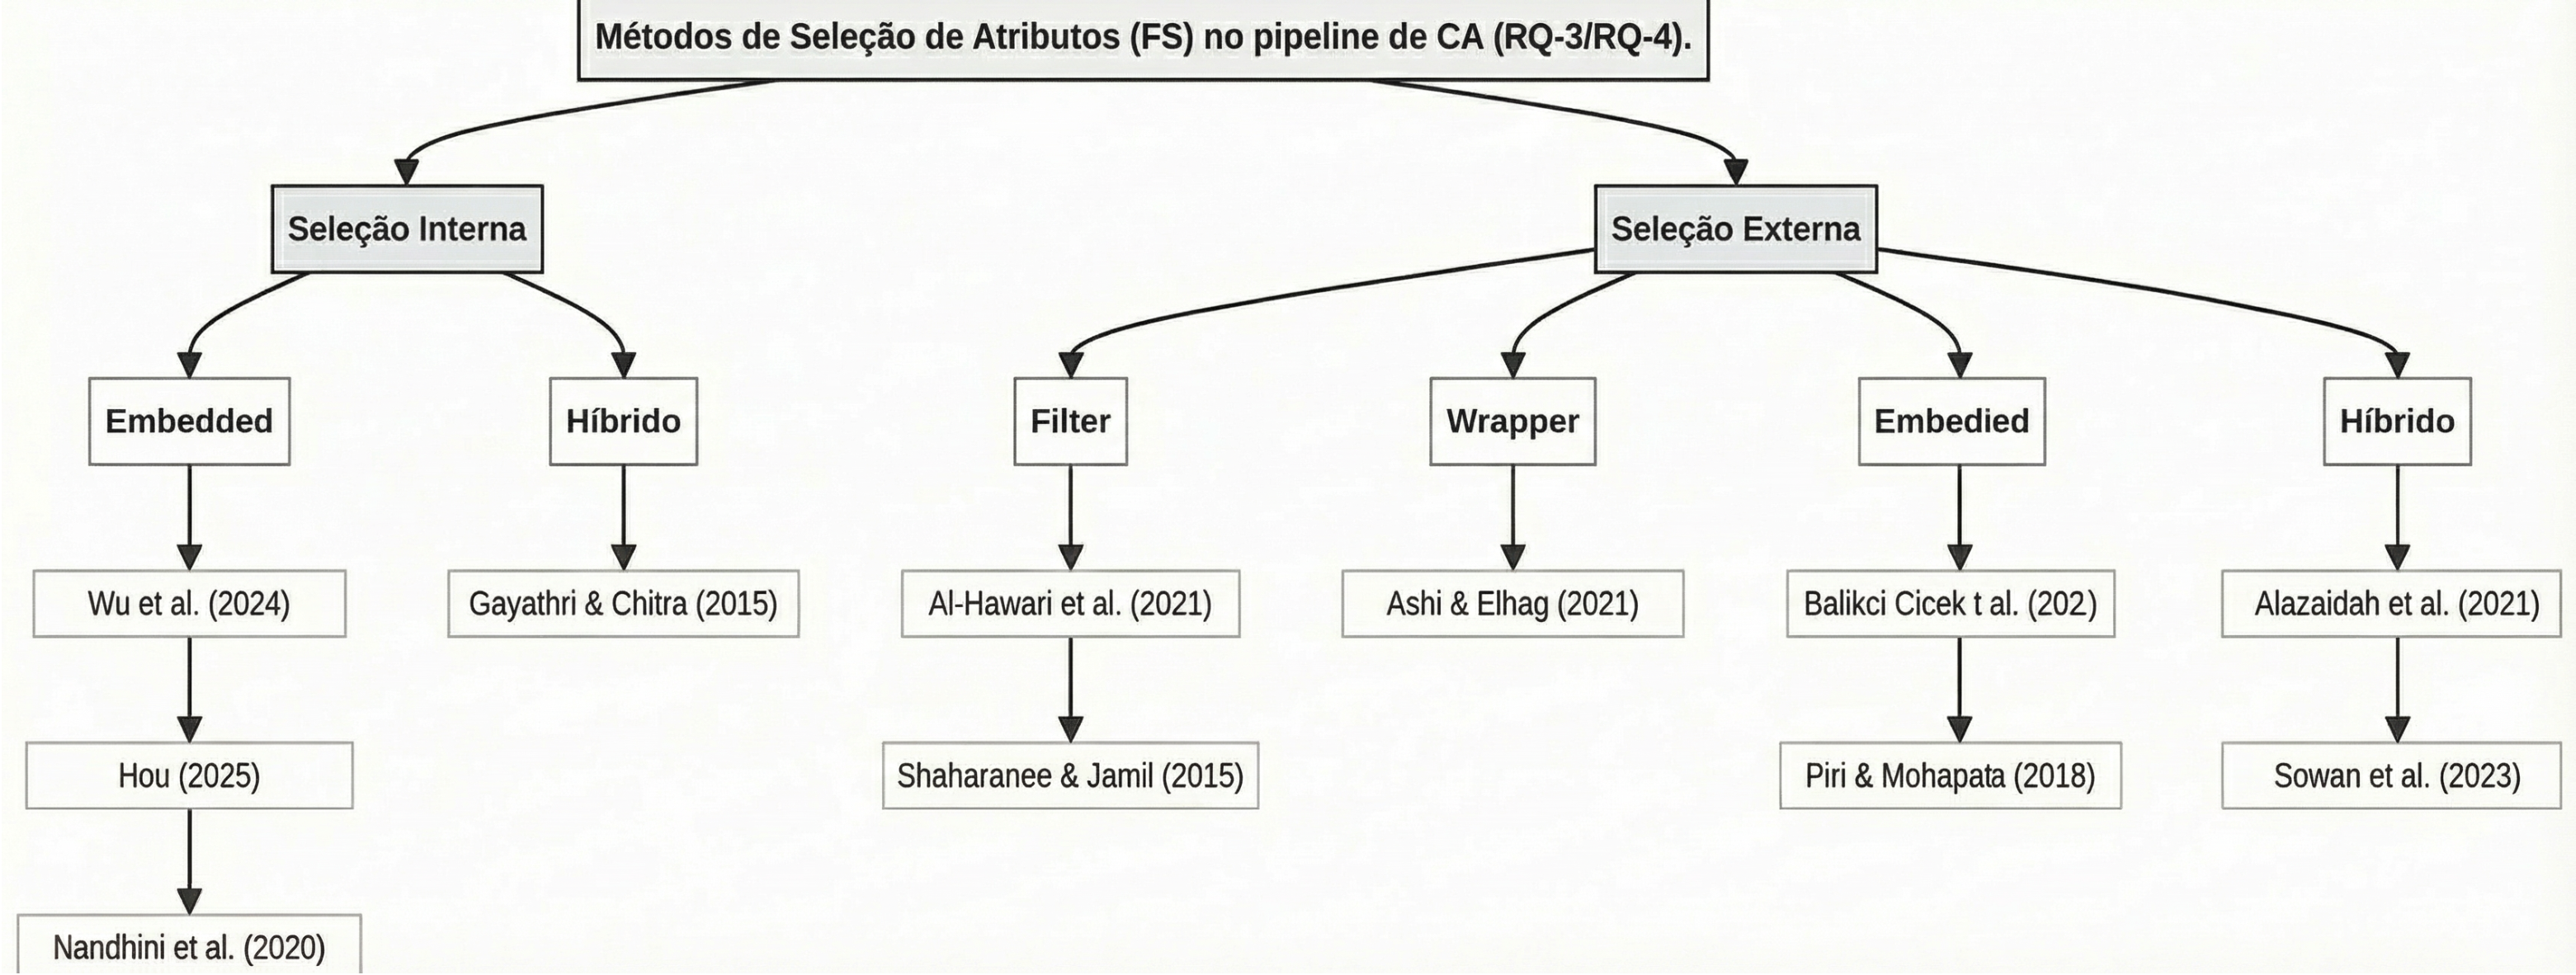
\includegraphics[width=\textwidth]{figuras/taxonomia_hierarquica.png}
\caption{Métodos de Seleção de Atributos (FS) no pipeline de CA, organizados por forma de inserção (interna/externa) e por tipo metodológico (filter, wrapper, embedded e híbrido).}
\label{fig:rq3_rq4_fs}
\end{figure}

A Figura~\ref{fig:rq3_rq4_fs} oferece uma visão taxonômica do corpus: de um lado, estudos em que a FS é parte estrutural do próprio classificador associativo; de outro, trabalhos em que a FS atua como etapa anterior de redução do espaço de atributos. Essa distinção é central porque não se trata apenas de \emph{quando} selecionar atributos, mas de \emph{com que papel} a seleção interfere no processo de mineração de regras.

\subsubsection{Discussão das RQ-3 e RQ-4}

Os estudos analisados se distribuem em dois desenhos metodológicos claramente distintos. No primeiro, a FS é aplicada como \textbf{etapa externa ao classificador}, geralmente no pré-processamento. No segundo, a FS é \textbf{interna ao pipeline de CA}, isto é, incorporada à própria lógica de indução, ponderação, mineração ou poda de regras.

\paragraph*{RQ-3: Inserção da FS no pipeline de CA.}
A predominância mais evidente no corpus é a da \textbf{seleção externa}. Nessa configuração, a FS ocorre antes da mineração de regras ou da construção do classificador, com o objetivo de reduzir dimensionalidade, eliminar atributos irrelevantes e tornar o espaço de busca mais controlável. Esse padrão aparece em \cite{alhawari2021classification}, \cite{ashi2021enhancing}, \cite{cicek2021assessment}, \cite{piri2019exploring}, \cite{alazaidah2021feature}, \cite{sowan2023hybrid} e \cite{shaharanee2015irrelevant}. Em termos práticos, trata-se de um desenho pipeline clássico: dados brutos $\rightarrow$ pré-processamento/discretização $\rightarrow$ FS $\rightarrow$ mineração de regras/classificação.

Esse arranjo externo, contudo, não é homogêneo. Em \cite{alhawari2021classification}, a FS atua sobre dados textuais ainda na representação de termos, filtrando palavras relevantes por \textit{Information Gain} e $\chi^2$ antes da classificação de reviews em tarefas de manutenção. Em \cite{cicek2021assessment}, a FS é usada para reduzir um espaço genômico de alta dimensionalidade via \textit{LASSO}, isto é, por regularização, antes da aplicação do classificador associativo. Já em \cite{piri2019exploring}, a redução ocorre após a discretização e antes da mineração, por meio da importância de atributos estimada com \textit{ExtraTreesClassifier}. Em \cite{shaharanee2015irrelevant}, a FS externa é ainda mais explicitamente conectada à mineração de regras: primeiro removem-se atributos irrelevantes por \textit{Symmetrical Tau} ou \textit{Mutual Information}; em seguida, removem-se também regras que contenham atributos descartados. Ou seja, a FS não apenas reduz atributos, mas reorganiza o próprio universo de regras possíveis.

Também há casos em que a FS externa é usada de forma comparativa e metodologicamente mais ampla. Em \cite{alazaidah2021feature}, o objetivo não é propor um único pipeline original de AC, mas comparar famílias distintas de FS --- \textit{filter}, \textit{wrapper} e heurísticas híbridas --- acopladas a classificadores associativos. Em \cite{sowan2023hybrid}, a FS externa é estruturada em dois estágios: um \textit{ensemble filter} (WARF), seguido de uma busca \textit{wrapper} com PSO, antes da classificação associativa. Nesse caso, a FS deixa de ser uma etapa simples e passa a ser um subsistema de otimização próprio.

Em contraste, a \textbf{seleção interna} aparece em menos estudos, mas com integração metodológica mais forte com a CA. Esse padrão ocorre em \cite{wu2024novel}, \cite{gayathri2015efficient}, \cite{hou2025improved} e \cite{nandhini2020performance}. Aqui, a FS não está separada do classificador: ela é absorvida pela própria mecânica de geração, avaliação ou ranqueamento de regras.

Em \cite{wu2024novel}, por exemplo, a FS é embutida na mineração ponderada de itemsets e regras do MCWCAR. A seleção de combinações de atributos ocorre durante a mineração, via \textit{mutual information weighted support}, enquanto a relevância item--classe é refinada por coeficiente de correlação. Não há um corte nítido entre “selecionar atributos” e “minerar regras”; ambas as tarefas são tratadas conjuntamente. Em \cite{gayathri2015efficient}, a integração ocorre por meio do critério BSIC, que calcula informação compartilhada entre atributos e padrões de doença, articulado com uma matriz de seleção e uma estratégia \textit{greedy} para evitar descarte de atributos importantes. Em \cite{hou2025improved}, a FS interna aparece associada ao cenário \textit{multi-label}, combinando importância de rótulos, seleção de atributos e mineração eficiente com FP-tree e poda local. Já em \cite{nandhini2020performance}, a FS está dentro do próprio gerador de regras do CPAR: os atributos do antecedente são escolhidos iterativamente por uma medida de ganho, o que caracteriza uma seleção \emph{on-the-fly} durante a indução.

Assim, a resposta à RQ-3 é que a FS aparece em \textbf{duas arquiteturas principais}: uma arquitetura \textbf{externa}, mais modular e compatível com pipelines tradicionais de pré-processamento; e uma arquitetura \textbf{interna}, mais fortemente acoplada ao raciocínio associativo e ao processo de indução das regras. A primeira prioriza controle da dimensionalidade antes da mineração; a segunda busca alinhar a seleção de atributos ao próprio mecanismo de descoberta de conhecimento.

\paragraph*{RQ-4: Métodos de FS empregados.}
Quanto aos métodos propriamente ditos, o corpus apresenta quatro grupos principais: \textbf{filter}, \textbf{wrapper}, \textbf{embedded} e \textbf{híbrido}. A Figura~\ref{fig:rq3_rq4_fs} resume essa organização, mas a análise detalhada mostra diferenças relevantes dentro de cada grupo.

Os métodos \textbf{filter} aparecem sobretudo nos estudos com seleção externa. Em \cite{alhawari2021classification}, a combinação de \textit{Information Gain} e $\chi^2$ é aplicada ao contexto de mineração de reviews, onde a unidade analítica são termos textuais. Aqui, FS significa ranquear palavras por relevância discriminativa. Em \cite{shaharanee2015irrelevant}, o contraste entre \textit{Symmetrical Tau} e \textit{Mutual Information} mostra duas leituras distintas de relevância: uma mais estatístico-heurística e outra mais informacional. Em ambos os casos, a lógica é a mesma: reduzir o espaço antes da mineração com custo computacional relativamente baixo.

Os métodos \textbf{wrapper} são menos frequentes, porém metodologicamente mais caros. Em \cite{ashi2021enhancing}, o método SBS-IEP-FS usa \textit{Sequential Backward Search} com a função de avaliação \textit{Inconsistent Examples Pairs}. Trata-se de uma busca explícita por subconjuntos, na qual a qualidade da seleção depende do desempenho avaliado ao longo do processo. Em \cite{alazaidah2021feature}, wrappers como ABB-IEP, ABB-LIU, SFS-IEP, SFS-LIU, SBS-IEP e SBS-LIU são comparados com filtros e heurísticas, evidenciando que o desempenho da FS em AC também depende das características dos dados e do algoritmo acoplado.

Os métodos \textbf{embedded} formam um grupo particularmente importante no corpus. Em \cite{cicek2021assessment}, a incorporação da FS ocorre por regularização \textit{LASSO}, zerando coeficientes e preservando apenas genes relevantes. Em \cite{piri2019exploring}, a importância das variáveis é produzida por um comitê de árvores (\textit{ExtraTreesClassifier}), e a seleção decorre diretamente do modelo. Já nos estudos com FS interna, o caráter \textit{embedded} é ainda mais claro: \cite{wu2024novel} incorpora pesos por MI e correlação no próprio processo de mineração; \cite{hou2025improved} utiliza importância de rótulos e seleção multi-rótulo; e \cite{nandhini2020performance} explora a escolha incremental de atributos do antecedente por medidas como FOIL’s Information Gain, Gain Ratio e Mutual Information Gain. Nesses casos, o método de FS não é um bloco separado do classificador, mas parte do próprio mecanismo de construção das regras.

Por fim, os métodos \textbf{híbridos} aparecem como tentativa de combinar baixo custo dos filtros com maior capacidade discriminativa dos wrappers ou mecanismos internos. Em \cite{gayathri2015efficient}, o BSIC-AC é híbrido porque une um critério Bayesiano de informação compartilhada com uma estratégia \textit{greedy}, buscando reduzir dimensão sem perder atributos relevantes. Em \cite{sowan2023hybrid}, o hibridismo é ainda mais explícito: o método WARF agrega vários filtros (CFS, IG, Gain Ratio, $\chi^2$, ReliefF) em um \textit{ensemble} ponderado; depois, o PSO opera como mecanismo de busca \textit{wrapper} sobre esse espaço reduzido. Em \cite{alazaidah2021feature}, o caráter híbrido aparece no próprio desenho comparativo do estudo, que reúne métodos de naturezas distintas no contexto da classificação associativa.

Em termos analíticos, os resultados das RQ-3 e RQ-4 mostram que a literatura não trata FS apenas como uma etapa acessória. Na prática, há dois grandes projetos metodológicos em disputa. O primeiro vê a FS como \textbf{pré-condição para viabilizar a CA}, sobretudo em cenários de alta dimensionalidade, texto ou genômica. O segundo vê a FS como \textbf{parte constitutiva do próprio processo associativo}, isto é, como um mecanismo que deve ser integrado à mineração e à avaliação das regras. O primeiro projeto favorece modularidade, simplicidade de implementação e redução do custo computacional; o segundo favorece maior coerência entre seleção de atributos e descoberta de regras discriminativas.

De forma sintética, os \textit{filters} externos tendem a ser adotados quando se busca redução rápida do espaço de atributos com menor custo computacional; os \textit{wrappers} e métodos híbridos perseguem subconjuntos mais discriminativos, embora com maior custo; e as abordagens \textit{embedded}/internas se destacam quando o objetivo é alinhar a seleção de atributos ao próprio processo de geração, ponderação, poda ou ranqueamento de CARs. Portanto, a evidência do corpus sugere que a escolha do método de FS em CA não depende apenas da família algorítmica, mas também do tipo de dado, do grau de dimensionalidade, da estrutura do problema de classificação e do nível de integração desejado entre FS e mineração de regras.

%%%%%%%%%%%%%%%%%%%%%%%%%%%%%%%%%%%%%%%%%%%%%%%%%%%%%%%%%%%%
\subsection{RQ-5 (Estratégias): Mitigação de Desbalanceamento além de FS}
%%%%%%%%%%%%%%%%%%%%%%%%%%%%%%%%%%%%%%%%%%%%%%%%%%%%%%%%%%%%

Esta questão identifica estratégias adicionais (além de FS) que atuam sobre (i) a mineração de itemsets/regras, (ii) o ranqueamento/seleção e (iii) a poda/decisão do classificador, visando reduzir viés em favor da classe majoritária e/ou controlar a explosão de regras em cenários desbalanceados.

\begin{table}[H]
\centering
\footnotesize
\setlength{\tabcolsep}{4pt}
\renewcommand{\arraystretch}{1.15}
\caption{RQ-5: Estratégias adicionais para mitigar desbalanceamento (além de FS) e respectivas medidas objetivas.}
\label{tab:rq5}
\begin{tabularx}{\textwidth}{|p{3.2cm}|p{3.6cm}|>{\raggedright\arraybackslash}X|}
\hline
\textbf{Estudo} & \textbf{Estratégias além de FS} & \textbf{Operacionalização / Medidas objetivas (IM/MO)} \\
\hline
Wu et al. \cite{wu2024novel} &
Custo-sensibilidade + limiares por objetivo + medida assimétrica &
(1) Mineração com \textbf{pesos} e \textbf{múltiplos suportes ponderados} por tipo de itemset (defeituoso, não-defeituoso, e associações entre atributos). (2) Substituição de suporte/confiança por \textbf{Added Value (AV)} para geração, ranqueamento e poda de CARs. (3) Predição por agregação (soma) de evidências via AV por classe. \\
\hline
Hou \cite{hou2025improved} &
Multiaprendizado do treino + limiar de interesse + força de regra &
(1) Extração múltipla do conjunto de treino para reduzir redundância e aumentar robustez. (2) Filtragem por \textbf{interest threshold} e \textbf{confidence threshold}. (3) Uso explícito de medidas de associação/força como \textbf{lift} e métricas derivadas para quantificar qualidade da regra e apoiar poda/filtragem. \\
\hline
Gayathri \& Chitra \cite{gayathri2015efficient} &
Poda do classificador + heurística \textit{greedy} para reduzir FPR &
(1) \textbf{Optimized Associative Classifier (OAC)} para \textbf{poda} de regras (subconjunto “pruned”). (2) Seleção \textit{greedy} baseada em \textbf{Total Compatible Length (TCL)} (com estrutura tipo árvore binária), com objetivo explícito de reduzir \textbf{false positive rate} e overfitting; seleção das “melhores” regras após a poda. \\
\hline
Al-Hawari et al. \cite{alhawari2021classification} &
Engenharia de \textit{interestingness} para seleção/decisão de CARs &
ACRM: extração/seleção de CARs guiada por \textbf{confiança} e \textbf{conviction}. Critério de decisão: regra de maior confiança; em empate (mesma confiança), usa-se \textbf{conviction} para desempate, melhorando consistência da decisão em multi-classes e reduzindo ambiguidade de regras concorrentes. \\
\hline
Ashi \& Elhag \cite{ashi2021enhancing} &
Suporte por classe + pós-processamento evolutivo (regras fuzzy) &
(1) Uso de \textbf{CBA2} como baseline \textbf{multi-minsup} (minsup por classe conforme distribuição). (2) No \textbf{FARC-HD}, \textbf{pré-triagem} de regras com métrica ponderada (ex.: \textit{wWRAcc}) e \textbf{seleção/ajuste por Algoritmos Genéticos} (regra e parâmetros), visando \textbf{reduzir número de regras} e simplificar antecedentes. \\
\hline
Nandhini et al. \cite{nandhini2020performance} &
Estimativa de erro + seleção das melhores $k$-regras &
No CPAR e variantes: (1) seleção de literais guiada por medidas de ganho (\textbf{FOIL-IG} e alternativas como \textbf{GR} e \textbf{IG}). (2) Avaliação/ranqueamento de regras por \textbf{Laplace accuracy (La)} e \textbf{Likelihood ratio (Lr)}. (3) Predição com \textbf{best-$k$ rules}, reduzindo o impacto de regras fracas/espúrias e controlando complexidade. \\
\hline
Shaharanee \& Jamil \cite{shaharanee2015irrelevant} &
Remoção de regras irrelevantes (pós-mineração) baseada em significância &
A estratégia visa impedir que regras “contaminadas” por atributos irrelevantes dominem o conjunto final: (1) determinação de relevância de atributos via \textbf{Symmetrical Tau (ST)} e comparação com \textbf{Mutual Information (MI)}; (2) mineração/pós-filtro para eliminar regras compostas por atributos não significativos, mantendo \textbf{cobertura} e evitando explosão de regras irrelevantes. \\
\hline
\end{tabularx}
\end{table}

\subsubsection{Discussão RQ-5:}
Em conjunto, os estudos convergem para um padrão: ao invés de reamostragem explícita, a mitigação do desbalanceamento é majoritariamente tratada por \textbf{engenharia do processo de mineração e seleção de regras}, isto é, ajustando (i) como regras são geradas (limiares/ponderações), (ii) como são avaliadas (IM/MOs mais informativas) e (iii) como são selecionadas/podadas (heurísticas e estimadores de erro).

No nível de mineração, destacam-se estratégias \textbf{classe-dependentes}. Em predição de defeitos, Wu et al. empregam \textbf{custo-sensibilidade} com \textbf{múltiplos limiares de suporte ponderado} por objetivo de mineração (minoria/maioria/associações), evitando que a baixa frequência da minoria inviabilize a geração de regras úteis. Em churn, a lógica de \textbf{multi-minsup por classe} (CBA2) aparece como mecanismo clássico para equilibrar a quantidade/qualidade de regras extraídas em distribuições assimétricas.

No nível de avaliação e decisão, observa-se a preferência por medidas que atacam limitações de suporte/confiança em cenários desbalanceados. Wu et al. substituem medidas simétricas/positivas por \textbf{AV} (assimétrica e sensível a associações negativas), aplicando-a consistentemente em geração, poda e predição. Em textos curtos e multi-classes, Al-Hawari et al. usam \textbf{conviction} como critério complementar à confiança para reduzir ambiguidades entre regras concorrentes (mesma confiança, classes distintas). Hou reforça esse eixo ao propor filtragem por \textbf{limiar de interesse} e métricas de associação (p.ex., \textbf{lift}) para selecionar regras mais “informativas” e reduzir redundância.

Por fim, no nível de poda/compactação, há três linhas fortes: (i) \textbf{poda direta do conjunto de regras} (OAC + seleção \textit{greedy} por TCL em BSIC-AC), atacando FPR/overfitting; (ii) \textbf{seleção baseada em estimativa de erro e best-$k$ rules} (La/Lr no CPAR), reduzindo influência de regras fracas; e (iii) \textbf{pós-processamento evolutivo} (FARC-HD), que combina pré-triagem por métrica ponderada e seleção/tuning por GA para produzir modelos mais compactos. Em paralelo, a remoção explícita de regras irrelevantes (Shaharanee \& Jamil) atua como salvaguarda para evitar que atributos pouco informativos inflacionem o conjunto de regras, preservando cobertura e simplificando o modelo.

%%%%%%%%%%%%%%%%%%%%%%%%%%%%%%%%%%%%%%%%%%%%%%%%%%%%%%%%%%%%
\subsection{RQ-6 (Avaliação): Protocolos e Métricas}
%%%%%%%%%%%%%%%%%%%%%%%%%%%%%%%%%%%%%%%%%%%%%%%%%%%%%%%%%%%%

A RQ-6 analisa o rigor experimental e a adequação das métricas ao contexto (inclusive desbalanceado),
considerando: (i) protocolo de validação (partição/reamostragem), (ii) métricas preditivas (globais e/ou
robustas a viés), (iii) métricas/IMs de regras usadas na indução (\textit{rule selection}) e (iv) custo/complexidade
(nº de regras/atributos e tempo), quando reportados.

\begin{table}[H]
\centering
\footnotesize
\setlength{\tabcolsep}{4pt}
\renewcommand{\arraystretch}{1.15}
\caption{Protocolos, métricas e evidências de rigor experimental (RQ-6).}
\label{tab:rq6}
\begin{tabularx}{\textwidth}{|p{3.1cm}|p{3.7cm}|p{2.2cm}|X|}
\hline
\textbf{Estudo} & \textbf{Comparativos} & \textbf{Protocolo} & \textbf{Métricas/Análises reportadas} \\
\hline
Wu et al. \cite{wu2024novel} &
CWCAR, CBA3, ACAR; comparação adicional com KPWE e GIS &
10$\times$5-fold CV (principal) + testes estatísticos &
\textbf{Pred.:} Balance (métrica principal), G-Mean, MCC, F-measure.
\textbf{IM/MO (regras):} Added Value (AV) na geração/seleção de CARs.
\textbf{Rigor:} Scott-Knott ESD (e comparação não-paramétrica) para diferenças entre métodos. \\
\hline
Gayathri \& Chitra \cite{gayathri2015efficient} &
DD-MSM, GIA-RST &
Experimentos (Java; reamostragem/partição não explicitada) &
\textbf{Pred.:} Classification Accuracy (\%) e False Positive Rate (FPR).
\textbf{FS/Complex.:} evidência via redução de dimensão/tempo (quando reportado). \\
\hline
Hou \cite{hou2025improved} &
AC, IAMC, MLFS, FP-tree &
Experimentos por iteração (treino/teste; protocolo agregado) &
\textbf{Pred.:} erro de teste e erro de treino ao longo das iterações; erro global de classificação.
\textbf{Complex.:} tempo de execução/consumo e análise de eficiência (p.ex., resposta por tamanho amostral). \\
\hline
Balikci Cicek et al. \cite{cicek2021assessment} &
Sem baselines explícitos (foco em modelo AC no domínio) &
Protocolo não explicitado no texto (relato por resultados) &
\textbf{Pred.:} Accuracy, Balanced Accuracy, Sensitivity, Specificity, PPV, NPV e F1-score. \\
\hline
Al-Hawari et al. \cite{alhawari2021classification} &
NB, J48, SVM, GBT, RF; ACs (CBA, CBA2, CMAR, CPAR) + ACRM &
10-fold (usado nas varreduras/experimentos) &
\textbf{Pred.:} Precision, Recall, F-score e Accuracy (médias).
\textbf{IM/MO (regras):} comparação/seleção de IMs (p.ex., confidence e conviction; também testam Laplace/lift em experimento).
\textbf{Rigor:} testes com estatística Z, $p$-valor e tamanho de efeito (Cliff’s delta) quando aplicável. \\
\hline
Ashi \& Elhag \cite{ashi2021enhancing} &
CBA, CBA2, CPAR e FARC-HD &
10-fold CV (KEEL) + análise estatística &
\textbf{Pred.:} Accuracy e Error Rate; ROC (curva).
\textbf{Complex.:} tempo médio e número de regras.
\textbf{Rigor:} FriedmanAligned (rank) para comparação entre algoritmos. \\
\hline
Piri \& Mohapatra \cite{piri2019exploring} &
Comparação experimental (com e sem FS; comparativos de ML reportados) &
K-fold CV (K=10) &
\textbf{Pred.:} Accuracy (principal), comparando cenários com/sem FS.
\textbf{Complex.:} impacto da redução de atributos (quando discutido). \\
\hline
Alazaidah et al. \cite{alazaidah2021feature} &
CBA, CBA2 (msCBA), CFAR, CMAR, CPAR sob múltiplos FS &
10-fold CV (KEEL; metodologia comparativa) &
\textbf{Pred.:} Accuracy como métrica única de comparação entre FS$\times$AC.
\textbf{Obs.:} ausência de métricas robustas a desbalanceamento limita inferência em cenários enviesados. \\
\hline
Sowan et al. \cite{sowan2023hybrid} &
CBA e variações com filtros (IG/GR/$\chi^2$/ReliefF, etc.) + híbrido proposto &
10-fold CV &
\textbf{Pred.:} Accuracy (central; erro definido no artigo).
\textbf{Complex.:} nº de atributos selecionados e comparação com baselines (efeito do FS/PSO). \\
\hline
Shaharanee \& Jamil \cite{shaharanee2015irrelevant} &
Comparação de filtros (Symmetrical Tau vs Mutual Information) antes da mineração &
Treino vs teste em base ``unseen'' (proporção não explicitada) &
\textbf{Pred.:} Accuracy Rate (AR).
\textbf{Cobertura:} Coverage Rate (CR) (capacidade de cobrir instâncias).
\textbf{Complex.:} número de regras como proxy de explosão/interpretabilidade. \\
\hline
Nandhini et al. \cite{nandhini2020performance} &
CPAR clássico vs variantes (medidas de seleção/avaliação) &
10-fold CV e split 50:50 (cenário adicional) &
\textbf{Pred.:} Classifier Accuracy e AUC (ROC).
\textbf{IM/MO (regras):} uso de estimadores como Laplace e Likelihood Ratio em variantes/avaliação.
\textbf{Obs.:} inclui métrica mais robusta (AUC) frente a limiares e viés. \\
\hline
\end{tabularx}
\end{table}

\subsubsection{Discussão RQ-6:}
\textbf{(i) Protocolos e rigor.}
Há predominância de validação cruzada com $k{=}10$, mas com rigor desigual. Wu et al. \cite{wu2024novel}
se destacam por \textbf{repetição} (10$\times$5-fold) e por \textbf{testes estatísticos} (Scott-Knott ESD),
o que reduz conclusões dependentes de uma única partição. Já Ashi \& Elhag \cite{ashi2021enhancing}
também incorporam comparação estatística (FriedmanAligned), porém com foco em acurácia/erro e medidas operacionais.
Em contraste, Gayathri \& Chitra \cite{gayathri2015efficient}, Balikci Cicek et al. \cite{cicek2021assessment}
e Shaharanee \& Jamil \cite{shaharanee2015irrelevant} não explicitam completamente o protocolo de reamostragem,
o que limita reprodutibilidade e comparabilidade. Hou \cite{hou2025improved} reporta avaliação orientada a
\textit{erro/tempo} ao longo de iterações, mas sem detalhar um protocolo padrão (p.ex., CV estratificada).

\textbf{(ii) Métricas preditivas e adequação ao desbalanceamento.}
Somente uma parte dos estudos adota métricas explicitamente robustas a viés: Wu et al. \cite{wu2024novel}
priorizam \textbf{Balance} e reportam \textbf{G-Mean} e \textbf{MCC}; Balikci Cicek et al. \cite{cicek2021assessment}
incluem \textbf{Balanced Accuracy}, \textbf{Sensitivity} e \textbf{Specificity}; Nandhini et al. \cite{nandhini2020performance}
incluem \textbf{AUC}. Nos demais, a \textbf{acurácia} permanece central (ou única), como em Alazaidah et al.
\cite{alazaidah2021feature} e em Sowan et al. \cite{sowan2023hybrid}, o que é frágil quando há classe minoritária
relevante (pode inflar desempenho global e esconder baixa sensibilidade). Em texto, Al-Hawari et al.
\cite{alhawari2021classification} avançam ao usar Precision/Recall/F-score, aproximando a avaliação de erros assimétricos.

\textbf{(iii) Métricas de regras (IM/MO) e seleção.}
Alguns estudos tratam IM/MO como parte explícita da avaliação/indução. Wu et al. \cite{wu2024novel} usam
\textbf{Added Value} (AV) como medida assimétrica de valor adicional para regras sob viés. Em ACRM, Al-Hawari et al.
\cite{alhawari2021classification} comparam IMs (p.ex., \textbf{confidence} e \textbf{conviction}, e alternativas como
Laplace/lift em experimentos) para definir a seleção de CARs. Em BSIC-AC, Gayathri \& Chitra \cite{gayathri2015efficient}
operacionalizam a redução de \textbf{FPR} via critério de compatibilidade/seleção (\textit{greedy}), conectando FS e erro.

\textbf{(iv) Complexidade e interpretabilidade (regra-modelo).}
Como CA produz modelos por regras, é metodologicamente coerente reportar \textbf{número de regras} e/ou \textbf{tempo}.
Isso aparece com clareza em Ashi \& Elhag \cite{ashi2021enhancing} (tempo e nº de regras) e em Shaharanee \& Jamil
\cite{shaharanee2015irrelevant} (nº de regras + cobertura). Hou \cite{hou2025improved} enfatiza \textbf{tempo} e eficiência.
Onde tais medidas não aparecem, fica difícil julgar se ganhos preditivos vieram à custa de explosão de regras, prejudicando uso prático.

No conjunto, apenas uma fração dos estudos combina (a) protocolo robusto + (b) métricas adequadas ao viés + (c) análise de
complexidade. Para alinhamento com cenários desbalanceados, recomenda-se padronizar: CV estratificada (idealmente repetida),
métricas robustas (MCC/G-Mean/Balanced Accuracy/AUC) e sempre pelo menos uma medida de custo (nº de regras/tempo).
